\documentclass[UTF8, zihao=-4, a4paper, openany, fontset=none]{ctexrep}

\usepackage[
  a4paper,
  top=3.80cm,
  bottom=3.80cm,
  left=3.20cm,
  right=3.20cm,
  headheight=18pt,
  headsep=0.80cm,
  footskip=1.00cm
]{geometry}

\usepackage{fontspec}
\setCJKmainfont{Songti SC}
\setCJKsansfont{Heiti SC}
\setCJKmonofont{Songti SC}
\setCJKfamilyfont{song}{Songti SC}
\setCJKfamilyfont{hei}{Heiti SC}
\newcommand{\songti}{\CJKfamily{song}}
\newcommand{\heiti}{\CJKfamily{hei}}
\setmainfont{Times New Roman}

\usepackage{amsmath, amssymb}
\usepackage{graphicx}
\usepackage{booktabs}
\usepackage{longtable}
\usepackage{array}
\usepackage{calc}
\usepackage{caption}
\usepackage{fancyhdr}
\usepackage{tocloft}
\usepackage{enumitem}
\usepackage{microtype}
\usepackage[hidelinks]{hyperref}
\newcounter{none}
\makeatletter
\newsavebox\pandoc@box
\newcommand*\pandocbounded[1]{%
  \sbox\pandoc@box{#1}%
  \ifdim\wd\pandoc@box>\linewidth
    \resizebox{\linewidth}{!}{#1}%
  \else
    #1%
  \fi
}
\makeatother

\newcommand{\hqubodyfont}{\songti\fontsize{12pt}{21pt}\selectfont}
\AtBeginDocument{\hqubodyfont}
\setlength{\parindent}{2em}
\setlength{\parskip}{0pt}
\setlength{\emergencystretch}{3em}

\renewcommand{\thechapter}{\arabic{chapter}}
\renewcommand{\thesection}{\thechapter.\arabic{section}}
\renewcommand{\thesubsection}{\thesection.\arabic{subsection}}
\renewcommand{\thesubsubsection}{\thesubsection.\arabic{subsubsection}}
\setcounter{secnumdepth}{3}
\numberwithin{equation}{chapter}
\renewcommand{\theequation}{\thechapter-\arabic{equation}}
\renewcommand{\thetable}{\thechapter-\arabic{table}}
\renewcommand{\thefigure}{\thechapter-\arabic{figure}}

\ctexset{
  chapter = {
    name = {},
    number = \arabic{chapter},
    aftername = \quad,
    format = \centering\bfseries\songti\fontsize{16pt}{21pt}\selectfont,
    beforeskip = 24pt,
    afterskip = 18pt
  },
  section = {
    format = \bfseries\songti\fontsize{14pt}{21pt}\selectfont,
    beforeskip = 18pt,
    afterskip = 6pt
  },
  subsection = {
    format = \bfseries\songti\fontsize{12pt}{21pt}\selectfont,
    beforeskip = 12pt,
    afterskip = 6pt
  },
  subsubsection = {
    format = \songti\fontsize{12pt}{21pt}\selectfont,
    beforeskip = 6pt,
    afterskip = 0pt
  }
}

\setcounter{tocdepth}{2}
\renewcommand{\cftchapfont}{\songti\fontsize{12pt}{20pt}\selectfont\bfseries}
\renewcommand{\cftchappagefont}{\songti\fontsize{12pt}{20pt}\selectfont\bfseries}
\renewcommand{\cftsecfont}{\songti\fontsize{12pt}{20pt}\selectfont}
\renewcommand{\cftsecpagefont}{\songti\fontsize{12pt}{20pt}\selectfont}
\renewcommand{\cftsubsecfont}{\songti\fontsize{12pt}{20pt}\selectfont}
\renewcommand{\cftsubsecpagefont}{\songti\fontsize{12pt}{20pt}\selectfont}
\setlength{\cftbeforechapskip}{6pt}

\DeclareCaptionLabelFormat{hqulabel}{#1#2}
\DeclareCaptionLabelSeparator{hququad}{\quad}
\captionsetup{
  font={small},
  labelfont={bf},
  labelformat=hqulabel,
  labelsep=hququad,
  justification=centering
}
\captionsetup[table]{position=top}
\captionsetup[figure]{position=bottom}

\newcommand{\thesistitle}{工业机器人与劳动者重新配置}
\newcommand{\thesissubtitle}{来自中国微观数据的证据}
\newcommand{\thesiscollege}{经济与金融学院}
\newcommand{\thesismajor}{经济学}
\newcommand{\thesisgrade}{2022级}
\newcommand{\thesisstudentid}{20224105022}
\newcommand{\thesisauthor}{马浩宣}
\newcommand{\thesisadvisor}{杜宇洪 副教授}
\newcommand{\thesisdate}{2026年5月}
\newcommand{\thesisfulltitle}{\thesistitle —— \thesissubtitle}

\fancypagestyle{hqufront}{%
  \fancyhf{}
  \fancyhead[C]{\zihao{-5}\leftmark}
  \fancyfoot[C]{\zihao{-5}\thepage}
  \renewcommand{\headrulewidth}{0.4pt}
  \renewcommand{\footrulewidth}{0pt}
}

\fancypagestyle{hqumain}{%
  \fancyhf{}
  \fancyhead[L]{\zihao{-5}\thesistitle}
  \fancyhead[R]{\zihao{-5}华侨大学本科毕业论文}
  \fancyfoot[C]{\zihao{-5}\thepage}
  \renewcommand{\headrulewidth}{0.4pt}
  \renewcommand{\footrulewidth}{0pt}
}

\newcommand{\makehqucover}{%
  \clearpage
  \begingroup
  \newgeometry{top=2.50cm,bottom=2.50cm,left=3.00cm,right=2.50cm}
  \thispagestyle{empty}
  \centering
  
\includegraphics[width=2.6cm]{assets/hqu-emblem.png}\par
  \vspace{0.2cm}
  
\includegraphics[width=5.8cm]{assets/hqu-wordmark.png}\par
  \vspace{0.8cm}
  {\heiti\fontsize{20pt}{26pt}\selectfont 本科毕业论文（设计）\par}
  \vspace{1.2cm}
  {\heiti\fontsize{22pt}{30pt}\selectfont \thesistitle\par}
  \vspace{0.25cm}
  {\heiti\fontsize{18pt}{26pt}\selectfont —— \thesissubtitle\par}
  \vspace{1.5cm}
  {\zihao{3}
  \renewcommand{\arraystretch}{1.55}
  \begin{tabular}{|>{\centering\arraybackslash}p{3.2cm}|>{\centering\arraybackslash}p{8.5cm}|}
    \hline
    学\quad 院 & \thesiscollege \\
    \hline
    专\quad 业 & \thesismajor \\
    \hline
    年\quad 级 & \thesisgrade \\
    \hline
    学\quad 号 & \thesisstudentid \\
    \hline
    姓\quad 名 & \thesisauthor \\
    \hline
    指导老师 & \thesisadvisor \\
    \hline
  \end{tabular}\par}
  \vfill
  {\songti\zihao{-4}华侨大学教务处印制\par}
  \vspace{0.3cm}
  {\bfseries\zihao{-4}\thesisdate\par}
  \restoregeometry
  \endgroup
  \clearpage
}

\newcommand{\makeintegritypage}{%
  \clearpage
  \thispagestyle{empty}
  \begin{center}
    {\heiti\fontsize{16pt}{24pt}\selectfont 华侨大学本科毕业论文（设计）诚信承诺书}
  \end{center}
  \vspace{1.0cm}
  本人（姓名）\underline{\makebox[3.0cm]{\thesisauthor}}\quad
  学号\underline{\makebox[3.0cm]{\thesisstudentid}}\quad
  专业\underline{\makebox[3.0cm]{\thesismajor}}\par
  \vspace{0.5cm}
  郑重承诺：所呈交的毕业论文（设计）是在指导教师指导下自主完成。\par
  \vspace{0.3cm}
  论文题目：\underline{\makebox[8.6cm]{\thesisfulltitle}}\par
  \vspace{0.3cm}
  毕业论文（设计）选题和研究内容中不存在不正当引用、抄袭、伪造、篡改、代写、买卖等行为，如有违规行为，本人愿意承担一切责任。
  \vspace{2.0cm}
  \begin{flushright}
    承诺人（签名）：\underline{\makebox[4cm]{}}\\[1.2cm]
    年\quad 月\quad 日
  \end{flushright}
  \clearpage
}

\newenvironment{abstractzh}{%
  \clearpage
  \pagenumbering{Roman}
  \pagestyle{hqufront}
  \markboth{摘要}{摘要}
  \chapter*{\texorpdfstring{\heiti 摘\quad 要}{摘要}}
  \addcontentsline{toc}{chapter}{摘要}
}{\par}

\newcommand{\keywordszh}[1]{%
  \par\noindent\textbf{关键词：}#1\par
}

\newenvironment{abstracten}{%
  \clearpage
  \markboth{Abstract}{Abstract}
  \chapter*{Abstract}
  \addcontentsline{toc}{chapter}{Abstract}
}{\par}

\newcommand{\keywordsen}[1]{%
  \par\noindent\textbf{Keywords:} #1\par
}

\newcommand{\hqufronttoc}{%
  \clearpage
  \markboth{目录}{目录}
  \renewcommand{\contentsname}{\texorpdfstring{目\quad 录}{目录}}
  \tableofcontents
  \clearpage
  \pagenumbering{arabic}
  \pagestyle{hqumain}
}

\begin{document}

\makehqucover
\makeintegritypage

\begin{abstractzh}
工业机器人扩散不仅改变企业任务组织，也改变劳动者在收入、行业、职业层级和岗位适配关系中的位置。本文关注中国制造业智能化转型中，省级机器人暴露是否对应劳动者重新配置，并进一步观察这种配置变化是否伴随求职、岗位技能掌握和证书---岗位适配等调整。

本文匹配 CFPS 2020、2022 年个体数据、IFR 行业机器人数据和省级产业结构资料，构造省级工业机器人密度对数，并利用 2008 年省级行业就业份额与美国行业机器人运行存量构造 Bartik 工具变量。基准分析采用工具变量两阶段方法，估计机器人暴露与工资、制造业就业、职业层级和兼职就业之间的关系；CLDS 2016、2018 年合并样本用于补充观察劳动者调整过程。

基准结果显示，省级工业机器人密度对数的工具变量估计系数在工资方程中为 0.1994，在制造业就业方程中为 0.0798，在职业层级（ISEI 得分）方程中为 0.9995，均达到常规显著水平。这表明，在本文样本和变量口径下，机器人暴露较高地区的劳动者工资回报、制造业就业概率和职业层级指标呈正向变化。兼职就业系数为 -0.0162，显著性和稳健性弱于前三类结果。

CLDS 补充分析显示，机器人暴露标准化值与证书---岗位不匹配正相关，与掌握岗位技能所需时间类别负相关；是否找过工作呈弱正相关，是否参加技术培训和找工作时间（月字段）未呈现稳定变化。这些结果提示，机器人暴露下的劳动者重新配置还可能伴随资格适配和岗位技能掌握方面的变化。

本文的证据说明，工业机器人扩散的劳动力市场后果需要放在工资回报、制造业就业、职业层级、工作时间安排和岗位适配关系共同变化的框架中考察。相应政策可将智能制造升级同职业资格标准更新、模块化互补型技能培训和公共就业信息服务结合起来，以降低资格错配、技能转换和重新搜索带来的调整成本。

\keywordszh{工业机器人；劳动者重新配置；Bartik 工具变量；职业层级；岗位适配}
\end{abstractzh}

\begin{abstracten}
The diffusion of industrial robots changes not only firms' task organization but also workers' positions in income distribution, industry allocation, occupational hierarchy, and job fit. This paper studies whether provincial robot exposure is associated with worker reallocation in China's manufacturing upgrading, and whether such reallocation is accompanied by changes in job search, job-skill acquisition, and certificate-job fit.
Using CFPS 2020 and 2022 individual data, IFR industry robot data, and provincial industry structure information, this paper constructs the log of provincial industrial robot density and a Bartik instrument based on 2008 provincial industry employment shares and US industry robot stocks. The baseline analysis applies two-stage least squares to estimate the relationship between robot exposure and wages, manufacturing employment, occupational hierarchy, and part-time status. Pooled CLDS 2016 and 2018 data are used as supplementary evidence on adjustment-related variables.
The baseline results show that the instrumental-variable coefficient on log robot density is 0.1994 in the wage equation, 0.0798 in the manufacturing-employment equation, and 0.9995 in the occupational-hierarchy equation. These estimates indicate that, within the sample and variable definitions used in this paper, workers in provinces with higher robot exposure have higher wage returns, a higher probability of manufacturing employment, and higher ISEI scores. The coefficient on part-time status is -0.0162 and is less robust than the first three outcomes.
The CLDS supplementary analysis shows a positive relationship between standardized robot exposure and certificate-job mismatch, a negative relationship with the ordered category of time needed to master job skills, and a weak positive relationship with whether the worker has searched for a job. Technical training participation and the monthly search-time measure do not show stable changes.
These findings suggest that the labor-market consequences of industrial robots should not be interpreted only through employment displacement. They are better understood as worker reallocation involving wage returns, industry allocation, occupational hierarchy, and job fit. Policy responses can link intelligent manufacturing upgrading with updated occupational certification standards, modular complementary skills training, and public employment information services.

\keywordsen{Industrial Robots; Worker Reallocation; Bartik Instrumental Variable; Occupational Hierarchy; Job Fit}
\end{abstracten}

\hqufronttoc

\chapter{绪论}\label{ux7eeaux8bba}

\section{研究背景与意义}\label{ux7814ux7a76ux80ccux666fux4e0eux610fux4e49}

\subsection{选题背景}\label{ux9009ux9898ux80ccux666f}

中国制造业正处于由规模扩张转向质量提升、由传统要素投入转向智能化改造的阶段。政策层面，《``十四五''机器人产业发展规划》将机器人研发、制造和应用列为衡量科技创新和高端制造业水平的重要标志{[}34{]}。工业机器人由此成为制造业智能化转型中的重要技术载体。

国际机器人联合会（IFR）发布的 World Robotics 2025 报告显示，2024 年中国新安装工业机器人约 29.5 万台，占全球新安装量的 54\%，工业机器人运行存量约 200 万台{[}35{]}。机器人扩散已经不只是企业设备更新问题，还关系到制造业组织方式和岗位需求结构的变化。企业在引入机器人后，会重新安排部分生产任务、岗位分工和用工需求，劳动者可进入的岗位集合也随之发生变化。因此，产业升级问题需要同时讨论劳动者配置变化。

围绕机器人扩散的劳动力市场后果，既有研究并未得到单一方向的结论。Graetz and Michaels 强调机器人应用对生产率和增加值的提升作用{[}12{]}，Acemoglu and Restrepo 则指出机器人扩张可能在特定情境下挤压就业和工资{[}11{]}。中国研究也呈现出多维度特征：王永钦和董雯、李磊等分别从制造业上市公司和中国经验讨论机器人兴起的劳动力市场效应{[}9-10{]}；魏下海等从移民工作任务视角揭示城市劳动力市场重塑{[}1{]}；巫瑞等、屈小博和黄海进一步把机器人应用与技能升级、工资溢价和人机适配联系起来{[}3-4{]}。这些差异表明，机器人扩散的劳动力市场效应不能只看工资或就业，还要看收入回报、行业去向、职业位置和岗位适配状态的共同变化。

因此，仅从就业总量或平均工资出发，难以充分刻画工业机器人扩散的劳动力市场后果。工资回报反映收益分配，行业去向反映部门配置，职业位置反映任务和岗位层级，就业形态和岗位适配状态则反映劳动者工作安排、技能资格与岗位要求之间的关系。随着岗位任务、资格要求和工作组织方式发生变化，劳动者也可能面临新的调整成本和适配压力。

基于上述背景，本文关注的核心问题是：在中国制造业智能化转型持续推进的过程中，工业机器人应用如何影响劳动者的配置结果，并且这种变化是否伴随求职状态、岗位技能掌握和证书---岗位适配方面的调整。本文据此把机器人扩散的劳动力市场后果放到工资回报、行业去向、职业层级、就业形态和岗位适配状态中讨论。

\subsection{研究意义}\label{ux7814ux7a76ux610fux4e49}

理论层面，Graetz and Michaels、Acemoglu and Restrepo 以及魏下海等研究已从生产率、就业、工资和任务重组等角度积累了重要证据{[}1,11-12{]}。这些研究为理解机器人冲击提供了基础，但仅从就业数量或平均工资出发，仍难以说明劳动者在不同行业、岗位和职业层级之间如何调整。本文将工资回报、行业去向、职业层级和就业形态等配置结果，与求职、岗位技能掌握和证书---岗位适配等调整表现放在同一分析框架中，用于讨论机器人扩散如何影响劳动者重新配置过程。

现实层面，中国制造业正处于智能化转型与劳动力结构调整并行推进的阶段。工业机器人应用可能提高生产效率，也会改变部分岗位的任务内容、资格要求和收入回报。对这些变化进行经验分析，可以把政策讨论从设备更新延伸到劳动者调整环节：劳动者能否承接新岗位，职业资格能否反映岗位要求，培训和公共就业服务能否降低调整成本。本文据此识别机器人扩散后劳动者调整中更需要政策回应的环节。

\section{研究内容与研究方法}\label{ux7814ux7a76ux5185ux5bb9ux4e0eux7814ux7a76ux65b9ux6cd5}

\subsection{研究内容}\label{ux7814ux7a76ux5185ux5bb9}

围绕工业机器人扩散对劳动者重新配置的影响，本文依次回答三个问题。第一，机器人暴露是否改变劳动者的工资回报、制造业就业、职业层级和就业形态等配置结果。第二，如果配置结果发生变化，这些变化是否伴随求职状态、岗位技能掌握和证书---岗位适配等调整过程。第三，配置结果和调整过程合在一起，能够如何说明机器人扩散后的劳动者重新配置。

上述问题分别对应本文的基准分析和补充分析。基准分析识别配置结果变化，补充分析观察劳动者调整过程；具体数据分工和变量构造在第四章说明。

\subsection{研究方法}\label{ux7814ux7a76ux65b9ux6cd5}

本文将 IFR 行业机器人数据与中国微观调查数据相结合。由于机器人数据主要反映行业层面的自动化扩散，而劳动者调查数据记录个体层面的就业和岗位信息，本文依据历史地区产业结构，将行业机器人变化转换为省级机器人暴露指标。一个省份在机器人扩散较快行业中的历史就业份额越高，其劳动者面对的机器人暴露强度也越高。

考虑到机器人应用可能与地区产业基础、工资水平和劳动力市场条件同时相关，本文进一步构造 Bartik 工具变量。该工具变量利用外部行业层面的机器人变化与地区既有产业结构的结合，以降低地区同期劳动力市场条件反向影响机器人暴露的风险。基准分析考察工资回报、制造业就业、职业层级和就业形态等配置结果；补充分析观察求职、岗位技能掌握和证书---岗位适配等调整表现。

在经验估计上，本文以 IV-2SLS 为主，并结合 OLS、简约式估计、稳健性检验和扩展分析进行对照。这些结果用于判断机器人暴露与劳动者配置结果之间的经验关系，并说明结论在样本、模型设定和数据来源上的适用边界。

\section{研究思路与技术路线}\label{ux7814ux7a76ux601dux8defux4e0eux6280ux672fux8defux7ebf}

\subsection{研究思路}\label{ux7814ux7a76ux601dux8def}

本文以工业机器人扩散下劳动者重新配置为主线，从配置结果进入调整过程。收入表现、行业去向、职业位置和就业形态用于观察劳动者配置结果，岗位适配、技能掌握和求职状态用于观察调整过程中的相关线索。

本文先考察机器人暴露是否改变劳动者配置结果，再结合补充数据观察相关调整过程。首先，利用 CFPS 数据识别机器人暴露与劳动者工资回报、制造业就业、职业层级和就业形态之间的关系，回答机器人扩散是否改变劳动者配置结果。其次，利用 CLDS 数据观察求职、培训、岗位技能掌握和证书---岗位适配等变量，补充说明配置变化背后的调整线索。最后，结合主结果和补充分析，归纳机器人扩散后劳动者重新配置的主要表现及其解释范围。

\subsection{技术路线设计}\label{ux6280ux672fux8defux7ebfux8bbeux8ba1}

本文技术路线从研究问题出发。首先，在制造业智能化转型和工业机器人扩散背景下，提出劳动者重新配置问题。其次，结合任务重组和岗位匹配相关理论，形成``机器人暴露---配置结果---调整过程''的分析框架。再次，依据 IFR 行业机器人数据和历史地区产业结构构造省级机器人暴露指标。

在实证部分，本文先使用 CFPS 数据和 IV-2SLS 模型估计工资回报、制造业就业、职业层级和就业形态等配置结果，再通过稳健性检验和多年份扩展分析考察结果是否依赖特定样本或模型设定。随后，本文使用 CLDS 数据观察求职、培训、岗位技能掌握和证书---岗位适配等调整线索。最后，在上述结果基础上形成研究结论和政策建议。

\chapter{文献综述}\label{ux6587ux732eux7efcux8ff0}

\section{工业机器人与劳动力市场结果}\label{ux5de5ux4e1aux673aux5668ux4ebaux4e0eux52b3ux52a8ux529bux5e02ux573aux7ed3ux679c}

工业机器人扩散首先作用于企业任务组合和岗位需求。Autor、Levy 和 Murnane，Acemoglu and Autor，以及 Acemoglu and Restrepo 的任务框架研究表明，自动化会替代常规化、可编码任务，也可能通过生产率提升、产出扩张和新任务生成改变劳动需求{[}15,18-19{]}。Autor、Autor and Dorn 以及 Acemoglu and Restrepo 进一步将任务方法用于解释职业极化、服务岗位扩张和工资不平等变化{[}16,20-21{]}。因此，当常规任务收缩、互补岗位扩张和岗位要求调整同时发生时，机器人扩散的影响就不只表现为工资或就业总量变化，也会表现为劳动者在行业、职业层级和就业形态之间的重新分布。

国际研究对机器人劳动力市场影响的判断并不完全一致，这种差异与研究所观察的层次有关。Graetz and Michaels 基于跨国行业数据发现，机器人提高劳动生产率和增加值，但没有显著降低总就业{[}12{]}；Acemoglu and Restrepo 从美国地方劳动力市场出发，指出机器人扩张会压低就业和工资{[}11{]}；Kikuchi 等对日本的研究则强调自动化冲击下常规岗位收缩和职业结构重组{[}14{]}。上述研究说明，机器人冲击既可能体现为总量变化，也可能体现为岗位和职业结构调整。

中国研究进一步把视角推进到企业劳动需求、制造业就业、任务技能结构、工资回报和就业形态。李磊等、闫雪凌等和胡晟明等分别从企业需求、制造业就业和人力资本角度讨论机器人应用的劳动市场影响{[}6-7,10{]}；魏下海等强调机器人并未简单挤出城市劳动力，而是改变不同任务劳动者的城市就业机会{[}1{]}；巫瑞等、屈小博和黄海则把机器人应用与技能结构、人机适配和工资收益联系起来{[}3-4{]}；陈佳莹等进一步发现机器人使用可能提高非正规就业概率{[}2{]}。这些研究说明，机器人扩散下的劳动者重新配置需要同时从收入回报、行业去向、职业位置和就业形态观察。

在 CFPS 基准分析中，本文据此考察工资回报、制造业就业、职业层级和就业形态。工资回报对应劳动者收益变化，制造业就业对应行业配置，职业层级对应职业位置，就业形态对应劳动者参与劳动力市场方式。四类变量共同服务于本文对劳动者重新配置的经验观察。

\section{匹配效率、配置质量与岗位适配}\label{ux5339ux914dux6548ux7387ux914dux7f6eux8d28ux91cfux4e0eux5c97ux4f4dux9002ux914d}

在搜寻匹配理论中，劳动力市场匹配效率通常通过失业者、岗位空缺和新雇佣流量之间的关系来刻画。给定失业者数量 \(U\) 和岗位空缺数量 \(V\)，新雇佣流量 \(H\) 可写为：

\[
H=A \times m(U,V)
\]

其中，\(A\) 表示狭义匹配效率，即在给定失业者和岗位空缺规模下形成新雇佣关系的效率。Petrongolo and Pissarides、Hall and Schulhofer-Wohl 以及 Şahin et al.~主要依赖岗位空缺、雇佣流量和失业人口识别这一参数{[}25-27{]}；方福前等则使用失业持续期和招聘缺口刻画机器人应用下的短期匹配过程{[}8{]}。这类研究需要观察招聘和失业过程，本文使用的 CFPS 和 CLDS 数据主要记录劳动者侧的就业结果、岗位状态和调整经历。

基于这一概念边界，本文的经验分析转向劳动者侧可观察的配置结果和调整过程，具体包括收入回报、行业职业去向、就业形态和岗位适配等变化。

Jovanovic 把雇佣关系视为逐步发现的匹配过程{[}28{]}，Topel and Ward、Neal 则从工作转换、工资增长以及行业职业搜寻讨论流动中的匹配改善{[}29-30{]}。国内研究中，韩旭等也借助工作转换和工资增长观察城市规模与劳动力市场匹配质量之间的关系{[}5{]}。上述研究为从劳动者侧观察匹配质量提供了思路。受数据限制，本文不直接观察工作转换流量，而是结合工资回报、行业职业位置和 CLDS 状态变量，观察机器人暴露下劳动者配置和调整的相关变化。

机器人扩散还会改变岗位要求的技能组合、培训要求和证书---岗位适配关系。魏下海等、巫瑞等、屈小博和黄海均提示，机器人冲击与任务类型、技能结构和人机适配有关{[}1,3-4{]}。岗位要求变化可能带来技能吸收、资格适配和求职调整等过程，后文使用 CLDS 补充观察求职、岗位技能掌握、培训参与和证书---岗位适配等环节，具体题项和编码方式在变量构造部分说明。

\section{文献述评}\label{ux6587ux732eux8ff0ux8bc4}

前两节文献显示，工业机器人与劳动力市场研究已经从就业总量扩展到工资回报、行业去向、职业位置和岗位适配状态。机器人扩散既可能改变劳动替代关系，也可能通过生产率变化、任务重组和行业调整影响劳动者的岗位适配。仅观察就业总量或平均工资，容易遮蔽劳动者在行业、职业层级、就业形态和岗位适配关系上的重新配置。因此，本文需要在总量效应之外处理三个问题：劳动者配置变化如何观察，严格匹配效率与本文经验对象如何区分，机器人暴露的识别如何安排。

总量指标可以呈现净效应，但不能说明劳动者流向哪些行业、职业层级和就业形态。Graetz and Michaels 强调机器人对生产率和增加值的促进作用{[}12{]}，Acemoglu and Restrepo 则指出机器人暴露可能对地方就业和工资产生负向影响{[}11{]}。Dauth 等、Kikuchi 等和 Giuntella 等进一步从行业、职业、工时、培训和家庭决策等角度讨论劳动者调整{[}13-14,17{]}。这些研究共同说明，机器人扩散的劳动力市场后果应同时从总量变化和配置调整两方面理解。

中国研究进一步说明，机器人应用与任务、技能和岗位适配关系密切。李磊等从企业需求和产出扩张讨论就业效应{[}10{]}，魏下海等从移民工作任务视角强调机器人冲击下不同任务劳动者的就业机会差异{[}1{]}，巫瑞等和屈小博、黄海则把机器人应用与技能升级、工资溢价和人机适配联系起来{[}3-4{]}。陈佳莹等发现机器人使用与非正规就业概率上升相关{[}2{]}，说明就业形态也是配置调整的一部分。现有研究已经为理解机器人冲击提供了不同侧面，但较少把工资回报、行业去向、职业层级、就业形态和岗位适配放在同一劳动者侧配置框架下讨论。

严格匹配效率与本文讨论的劳动者重新配置属于不同分析层次。方福前等以失业持续期和招聘缺口刻画机器人应用下的短期匹配过程{[}8{]}，研究对象更接近搜寻匹配理论中的匹配效率。本文则将匹配效率作为概念边界，转向考察劳动者侧的配置结果与调整过程。

现有研究还提示，机器人采用本身可能与地区产业基础和劳动力市场条件相关。Acemoglu and Restrepo 以及 Goldsmith-Pinkham 等、Borusyak 等关于 shift-share 工具变量的研究说明，机器人暴露指标需要处理行业冲击与地区产业结构之间的关系{[}11,22-24{]}。后文将在研究设计中说明如何依据历史产业结构和外部行业冲击构造机器人暴露及其工具变量。

相对于既有文献，本文的增量不是重新估计匹配函数效率参数，而是在劳动者侧观察机器人暴露对应的配置结果和调整线索。本文所说的``劳动者重新配置''，是指自动化冲击下劳动者在收入、行业去向、职业位置、就业形态和岗位适配关系等方面的可观测配置变化。

\chapter{理论基础与研究假设}\label{ux7406ux8bbaux57faux7840ux4e0eux7814ux7a76ux5047ux8bbe}

\section{任务重组与劳动者重新配置}\label{ux4efbux52a1ux91cdux7ec4ux4e0eux52b3ux52a8ux8005ux91cdux65b0ux914dux7f6e}

工业机器人对劳动力市场的影响首先体现为生产任务组合的变化。自动化设备进入生产过程后，部分常规化、可编码任务被替代或重新组合，设备运维、流程控制、质量检验和跨环节协调等任务的重要性上升。Autor、Levy 和 Murnane，Acemoglu 和 Autor，以及 Acemoglu 和 Restrepo 的任务框架说明，机器人扩散首先改变企业需要哪些任务、岗位和技能{[}15,18-19{]}。

从劳动者配置看，任务重组至少会进入工资回报、行业去向和职业层级三个维度。生产率提升和互补任务扩张可能影响收入回报，机器人应用更集中的制造业部门可能改变劳动者行业去向，岗位任务复杂度变化则可能影响劳动者所处职业类别的社会经济地位。

在这些配置结果之外，技能要求和资格认证关系的调整还可能改变劳动者求职、培训、岗位技能掌握和证书---岗位适配关系。因此，本章先说明工资、行业和职业层级等配置结果，再说明求职、技能掌握和证书---岗位适配等调整过程。

\section{工业机器人影响劳动者配置的作用机制}\label{ux5de5ux4e1aux673aux5668ux4ebaux5f71ux54cdux52b3ux52a8ux8005ux914dux7f6eux7684ux4f5cux7528ux673aux5236}

\subsection{工资回报、行业配置与职业层级}\label{ux5de5ux8d44ux56deux62a5ux884cux4e1aux914dux7f6eux4e0eux804cux4e1aux5c42ux7ea7}

机器人通过任务重组改变劳动需求时，工资、行业去向和职业位置是最直接的观察维度。机器人可能替代部分常规任务，也可能通过生产率提升、新任务生成和互补型岗位扩张改变企业对劳动者的需求结构。Graetz and Michaels 发现机器人提高生产率和增加值{[}12{]}，Acemoglu and Restrepo 则指出机器人扩张可能压低就业和工资{[}11{]}，说明其净效应取决于替代效应、生产率效应和任务互补效应之间的相对强弱。工资、行业和职业层级因而构成本文观察配置结果的三个入口。

在工资回报维度上，工业机器人通过提高生产率并扩展互补性任务，改变企业劳动需求，进而影响劳动者工资回报。工业机器人进入生产过程后，部分标准化、重复性强的操作环节被设备吸收，设备运维、流程控制、质量检验、数据监测和跨环节协调等任务的重要性相对上升。当机器人提高生产效率并带来产出扩张时，能适应新任务结构的劳动者可能获得更高工资回报。因此，本文将工资收入对数指标理解为机器人冲击下收入回报变化的经验表现。

在行业配置维度上，制造业是工业机器人扩散最直接的承载部门，设备更新和生产组织再造会改变制造业内部及其相关环节的劳动需求。对于处在产业链扩张、订单增加或技术改造中的地区，机器人可能通过提高生产效率和稳定产品质量，增强制造业部门的岗位吸纳能力；技术维护、质量控制、生产管理和辅助服务岗位也可能随制造环节扩张而增加。由此，本文将是否处于制造业就业状态作为行业配置维度的观察指标，用以刻画劳动者是否更可能进入制造业部门；这一指标的解释还需要结合后文机器人暴露的行业来源分析。

在职业层级维度上，岗位任务复杂度变化可能影响劳动者职业位置。当企业内部常规任务被设备替代后，保留下来的岗位往往更强调设备协同、流程判断、质量控制、沟通协调和问题处理能力。这类任务要求的变化，可能提高部分劳动者进入较高社会经济地位职业类别的概率，也可能使职业位置差异扩大。因此，本文使用国际职业社会经济地位指数刻画职业层级变化，并将其理解为职业配置方向的结果指标。

除上述三类结果外，兼职就业作为附加维度，用于观察工作时间安排变化，不作为本文的核心配置结果。

工资回报、行业配置和职业层级分别对应机器人冲击下劳动者``收入是否变化''\,``是否流向制造业岗位''和``职业位置是否上移或分化''三个结果维度。多维结果框架可以避免把机器人影响简化为单一工资效应或单一就业效应。配置结果之外，还需要考察劳动者重新搜索、培训适应和证书---岗位适配的过程。

\subsection{求职摩擦与技能---岗位适配}\label{ux6c42ux804cux6469ux64e6ux4e0eux6280ux80fdux5c97ux4f4dux9002ux914d}

配置结果是地区劳动需求重排后的表现，调整摩擦则发生在劳动者重新搜索、学习和资格转换的过程中。工业机器人扩散会同时改变劳动者最终进入的岗位类型，以及岗位需求结构与劳动供给侧适应速度之间的关系。若岗位任务、技能要求和资格认证更新快于劳动者技能积累、证书转换和求职行为调整，那么即便配置结果发生变化，劳动者仍可能面临重新搜索、资格不匹配和技能适应压力。

韩旭等和 Şahin 等研究表明，岗位空缺与劳动供给在行业、职业或技能维度上的错位会影响工作找到率和匹配质量{[}5,27{]}。在机器人冲击情境下，这种错位主要体现为两类调整：一是劳动者是否需要重新搜索岗位，以及搜索过程是否伴随时间维度变化；二是岗位任务、岗位技能掌握和资格认证之间是否同步变化。本文据此从求职、培训、岗位技能掌握和证书---岗位适配四个环节观察劳动者调整过程。

这些调整变量的方向不必相同。流程标准化和任务重新拆分可能降低部分岗位的学习成本，资格认证、实际工作内容和技能结构不同步则可能提高证书---岗位不匹配。因此，本文在补充分析中观察工业机器人暴露与求职状态、培训参与、岗位技能掌握和证书---岗位适配之间的相关变化。

\section{理论命题与研究假设}\label{ux7406ux8bbaux547dux9898ux4e0eux7814ux7a76ux5047ux8bbe}

前文分析表明，工业机器人扩散会改变企业内部的任务结构和岗位需求。常规化、可编码任务被设备替代或重新组合，设备运维、流程控制、质量检验和跨环节协调等互补型任务的重要性上升。由此，机器人冲击既可能表现为工资、行业和职业层级等配置结果变化，也可能伴随重新搜索、技能吸收和资格适配等调整过程。据此，本文提出两个基准假设和两个补充分析命题。

\textbf{H1：工业机器人暴露与劳动者工资回报正相关。}
机器人应用可能通过提高生产率、扩大互补型岗位需求和改善部分岗位的劳动边际产出，提高劳动者获得工资回报的可能性。若生产率效应和互补岗位扩张占主导，机器人暴露较高地区的劳动者工资回报预期呈现上升趋势。

\textbf{H2：工业机器人暴露与制造业就业概率和职业层级正向变化相关。}
工业机器人首先在制造业及相关生产环节扩散，其带来的生产率提升和产业组织调整可能增强制造业岗位吸纳能力。同时，机器人应用会改变企业对操作、维护、协调和质量控制等任务的需求，进而影响劳动者进入不同职业类别的机会。因此，机器人暴露可能表现为制造业就业概率提高和职业层级指标变化。

H1 和 H2 对应 CFPS 基准估计中的配置结果。考虑到 CLDS 变量用于观察调整过程，本文进一步提出两个补充分析命题。

\textbf{H3：工业机器人暴露与劳动者求职状态变化相关。}
当岗位任务和技能要求发生变化时，部分劳动者需要在原有岗位、相近岗位和新岗位之间重新选择。机器人暴露较高的地区可能表现为是否找过工作这一状态变量的变化；找工作时间（月字段）仅作辅助观察，用于记录搜索过程是否伴随时间维度变化，其方向取决于岗位机会扩张和匹配摩擦的相对强弱。

\textbf{H4：工业机器人暴露与岗位技能掌握和证书---岗位适配变化相关。}
机器人扩散会改变岗位所需的操作知识、技术熟练度和资格要求。流程标准化可能降低部分岗位的学习成本，并改变掌握岗位技能所需时间类别；若流程标准化占主导，可能表现为类别下降。资格体系和实际工作内容更新不同步，则可能提高证书---岗位不匹配。培训需求和技术培训参与可作为辅助观察变量，用于补充刻画技能---岗位适配关系的变化。

上述假设对应本文的分层实证设计：CFPS 个体样本和 Bartik 工具变量用于检验机器人暴露对工资回报、行业配置和职业层级等配置结果的影响；CLDS 与省级机器人暴露变量用于补充观察求职、培训、岗位技能掌握和证书---岗位适配等过程变量的相关变化。由于机器人应用首先集中于制造业生产环节，实证部分还将对机器人暴露进行行业来源分析，用以说明基准结论主要反映何种产业冲击。

\chapter{研究设计}\label{ux7814ux7a76ux8bbeux8ba1}

\section{数据来源与样本说明}\label{ux6570ux636eux6765ux6e90ux4e0eux6837ux672cux8bf4ux660e}

本文使用两类微观调查数据和两类机器人暴露数据。CFPS 承担基准回归，CLDS 用于补充观察岗位适配与求职调整。这一分工对应前文的分析框架：CFPS 提供工资、行业、职业和工时信息，用于观察劳动者配置结果；CLDS 提供求职、培训、岗位技能掌握和证书---岗位适配信息，用于观察劳动者调整过程。

基准回归样本来自中国家庭追踪调查（China Family Panel Studies，CFPS）2020 年和 2022 年个人层面数据。CFPS 由北京大学中国社会科学调查中心组织实施，包含工资收入、就业行业、职业信息、工作时间，以及年龄、性别、受教育程度、城乡属性等基本特征，适合考察劳动者配置结果。本文以两期个人样本为基础，保留能够识别省份、调查年份并匹配省级机器人暴露变量的观测，构建个体---年份样本。匹配后的 CFPS 主样本覆盖 30 个省份，最大样本量为 34,315 个个体---年份观测，其中 2020 年为 17,796 个观测，2022 年为 16,519 个观测。工资、行业、职业和工作时间变量存在不同程度缺失，因此各结果变量进入回归时的有效样本量不同。

CFPS 用于构造个体结果变量和控制变量。工资收入来自个人问卷中的工作总收入字段，并在剔除非正收入后取对数；制造业就业根据行业编码识别；职业层级使用个人问卷中基于主要工作职业文本整理的 ISEI 分值；兼职就业根据每周工作时间构造。控制变量包括年龄、性别、受教育程度和城乡属性。为保持两期口径一致，2020 年和 2022 年的学历字段统一为 1---8 的序数量表；负值、拒答、不知道和不适用等调查缺失码按缺失值处理。上述变量的具体字段和构造规则在 4.2.2 与 4.2.4 节说明。

补充分析样本来自中国劳动力动态调查（China Labor-force Dynamics Survey，CLDS）2016 年和 2018 年个体数据。CLDS 由中山大学社会科学调查中心组织实施，包含岗位培训、岗位技能掌握、证书---岗位适配、是否找过工作等贴近劳动过程的变量。本文将 CLDS 2016 和 2018 合并为重复截面样本，将年龄限制在 16---60 岁，并保留能够匹配省份---年份机器人暴露的观测。该样本用于估计省级机器人暴露与培训需求、掌握岗位技能所需时间类别、技术培训参与、证书---岗位不匹配、是否找过工作和找工作时间（月字段）等过程变量之间的关系。上述 CLDS 变量的题项来源和编码处理在 4.2.3 节说明。该部分与 CFPS 基准回归相互补充，用于观察岗位适配和求职调整过程。

外部机器人暴露数据包括两类。第一类是省份---年份层面的工业机器人安装密度数据，用于构造核心解释变量；第二类是国际机器人联合会（International Federation of Robotics，IFR）的行业机器人数据，用于构造 Bartik 工具变量。本文将省级机器人安装密度取对数后作为机器人密度对数（ln\_robot），再以省份代码和年份为匹配键并入 CFPS 与 CLDS 个体样本。Bartik 工具变量利用基准期产业结构与美国行业机器人运行存量对数水平构造，用于缓解机器人暴露与地区劳动力市场条件同时变化带来的潜在内生性问题。

下文依次说明核心解释变量、结果变量、控制变量、工具变量和模型设定。

\section{变量选取与构造}\label{ux53d8ux91cfux9009ux53d6ux4e0eux6784ux9020}

\subsection{工业机器人暴露变量}\label{ux5de5ux4e1aux673aux5668ux4ebaux66b4ux9732ux53d8ux91cf}

核心解释变量为省级工业机器人密度对数（ln\_robot）。本文使用省份---年份层面的工业机器人安装密度衡量地区自动化渗透程度，该指标来自外部工业机器人安装密度数据，并按省份代码和年份与个体调查数据匹配。同一省份、同一年份的个体共享同一机器人暴露值，因此模型估计的是省级机器人暴露与个体配置结果之间的关系。Graetz and Michaels、Acemoglu and Restrepo 以及 Dauth 等通常使用 IFR 工业机器人数据构造国家、行业或地区层面的机器人暴露指标，以分析其对就业、工资和劳动力市场结构的影响{[}11-13{]}。中国情境下，魏下海等、屈小博和黄海也常将行业机器人信息与地区产业结构或就业结构结合，形成地区层面的机器人暴露度或机器人密度指标{[}1,4{]}。

变量构造上，机器人密度对数（ln\_robot）的基础变量为省份---年份层面的工业机器人密度，记为 \(RobotDensity_{pt}\)，其中 \(p\) 表示省份，\(t\) 表示年份。进入基准回归时，本文对该变量加 1 后取自然对数，构造为：

\[
ln\_robot_{pt}=\ln(1+RobotDensity_{pt})
\]

对数化处理有两方面考虑：一是机器人密度在不同省份之间差异较大，取对数可以降低极端值对估计结果的影响；二是对数形式便于解释机器人暴露强度变化与劳动力市场结果之间的关系。由于本文使用的是 \(\ln(1+RobotDensity_{pt})\)，机器人密度对数（ln\_robot）增加 1 表示 \(1+RobotDensity_{pt}\) 约提高为原来的 \(e\) 倍；在原始机器人密度较高时，可近似理解为机器人密度成比例上升。在不同结果方程中，其系数分别对应工资对数、就业概率、ISEI 得分或兼职概率的变化。在 CFPS 基准回归样本中，机器人密度对数为省级年度指标，2020 年和 2022 年个体样本分别匹配 2019 年和 2021 年的省级机器人暴露。后续模型据此把地区自动化冲击并入个体配置结果方程，并控制个体特征差异。

数据匹配上，本文以 CFPS 个体样本中的省份代码和调查年份为基础，将调查年前一年的省级机器人暴露变量匹配到个体层面。匹配完成后，同一省份---年份个体共享同一个机器人密度对数值；个体之间的差异则来自工资、行业、职业、工作时长以及年龄、性别、教育和城乡属性等微观变量。本文的识别对象是省级机器人暴露与个体配置结果之间的关系。

表4-1用于区分原始机器人暴露变量、进入回归的解释变量和 Bartik 工具变量。其中，robot\_density 为省级机器人密度的原始口径，ln\_robot 为进入基准模型的机器人暴露变量，bartik\_iv 由基准期省级行业就业份额与美国行业机器人运行存量加权构造，用于后续工具变量估计。

\textbf{表4-1 核心解释变量与工具变量构造}

{\def\LTcaptype{none} % do not increment counter
\begin{longtable}[]{@{}
  >{\raggedright\arraybackslash}p{(\linewidth - 6\tabcolsep) * \real{0.2500}}
  >{\raggedright\arraybackslash}p{(\linewidth - 6\tabcolsep) * \real{0.2500}}
  >{\raggedright\arraybackslash}p{(\linewidth - 6\tabcolsep) * \real{0.2500}}
  >{\raggedright\arraybackslash}p{(\linewidth - 6\tabcolsep) * \real{0.2500}}@{}}
\toprule\noalign{}
\begin{minipage}[b]{\linewidth}\raggedright
变量代码
\end{minipage} & \begin{minipage}[b]{\linewidth}\raggedright
变量名称
\end{minipage} & \begin{minipage}[b]{\linewidth}\raggedright
基本构造
\end{minipage} & \begin{minipage}[b]{\linewidth}\raggedright
模型角色
\end{minipage} \\
\midrule\noalign{}
\endhead
\bottomrule\noalign{}
\endlastfoot
robot\_density & 省级工业机器人密度 & RobotDensity\_\{pt\} & ln\_robot 的基础变量 \\
ln\_robot & 机器人密度对数 & ln(1 + RobotDensity\_\{pt\}) & 核心解释变量 \\
bartik\_iv & Bartik 工具变量 & Σ\_k share\_\{pk,2008\} × ln(1 + USRobot\_\{kt\}) & ln\_robot 的工具变量 \\
\end{longtable}
}

数据来源：工业机器人安装密度数据、IFR 工业机器人数据和 2008 年省级行业就业份额资料。

注：p、t 和 k 分别表示省份、年份和行业。上述变量按省份---年份匹配到个体样本；bartik\_iv 仅用于工具变量估计。

基于上述变量口径，本文进一步构建工具变量两阶段模型，以处理省级机器人暴露变量可能存在的内生性问题。

CLDS 补充分析使用省级机器人密度对数的标准化形式，具体口径见 4.3.4 节。

\subsection{配置结果变量（CFPS）}\label{ux914dux7f6eux7ed3ux679cux53d8ux91cfcfps}

本节界定 CFPS 基准回归中的被解释变量。本文基于 CFPS 个人问卷中的工作收入、行业、职业和工时题项，构造工资收入、制造业就业、职业层级和兼职就业四类结果变量。

第一类结果变量是工资收入对数（ln\_wage）。该变量来自 CFPS 个人问卷中的工作总收入题项。本文剔除缺失、拒答、不适用和非正收入记录后，对有效收入取自然对数。工资收入反映劳动者收入回报。

第二类结果变量是制造业就业（manu\_dummy）。该变量来自 CFPS 当前主要工作所属行业题项，依据行业编码判断劳动者是否处于制造业部门；当行业代码归属制造业时赋值为 1，行业信息有效且不属于制造业时赋值为 0。制造业是工业机器人应用最集中的部门，该变量反映劳动者行业去向。

第三类结果变量是职业层级（ISEI\_score）。该变量来自 CFPS 职业编码对应的国际职业社会经济地位指数（International Socio-Economic Index of Occupational Status，ISEI）。本文使用职业编码派生的 ISEI 分值，并将负值、无效编码和无法匹配 ISEI 分值的记录处理为缺失。ISEI 指数刻画职业类别在教育要求、收入位置和社会经济地位上的综合层级，数值越高表示职业社会经济地位越高{[}31{]}。

第四类结果变量是兼职就业（part\_time）。该变量来自 CFPS 每周工作时间题项。本文将每周工作时间低于 35 小时的劳动者定义为兼职就业并赋值为 1，每周工作时间达到或超过 35 小时的劳动者赋值为 0，工作时间缺失、无效或不适用的记录设为缺失。Callaghan and Hartmann 将兼职就业纳入 contingent work 的统计口径，并采用每周低于 35 小时识别兼职{[}32{]}；Koeber and Wright 则把全职失业者转向兼职再就业视为就业调整的一种表现{[}33{]}。本文据此将该变量作为工作时间安排和就业形态变化的辅助指标。

上述四类变量分别对应收入回报、行业去向、职业层级和工作时间安排。下一节说明 CLDS 中的求职、培训和资格适配变量。

\subsection{求职状态与岗位适配变量（CLDS）}\label{ux6c42ux804cux72b6ux6001ux4e0eux5c97ux4f4dux9002ux914dux53d8ux91cfclds}

CLDS 样本围绕求职、培训、岗位技能掌握和证书---岗位适配四类调整环节构造过程变量。与 CFPS 的工资、行业和职业结果相比，CLDS 变量更接近劳动者在岗位调整过程中的自报经历。

求职变量包括是否找过工作（searched\_recent）和找工作时间（月字段）（search\_months）。是否找过工作根据 CLDS 个体问卷中相关题项构造，回答``是''赋值为 1，回答``否''赋值为 0，负值、拒答和不知道等编码处理为缺失。找工作时间（月字段）来自求职时间题项中的月数字段，保留原始月数并处理异常编码；该变量没有将周、年字段统一折算为完整求职时长指标。

岗位适配相关变量包括当前岗位是否需要培训（need\_training）、掌握岗位技能所需时间类别（skill\_time）、是否参加技术培训（tech\_training）和证书---岗位不匹配（cert\_mismatch）。当前岗位是否需要培训来自对应题项，回答``是''赋值为 1，回答``否''赋值为 0。掌握岗位技能所需时间类别按原始有序时间类别保留，数值越大表示掌握岗位技能所需时间类别越高。是否参加技术培训根据技术培训题项构造，回答``是''赋值为 1，回答``否''赋值为 0。证书---岗位不匹配根据职业证书与岗位关系题项构造，证书与当前岗位不匹配赋值为 1，匹配赋值为 0；该变量在持有职业证书的样本中解释。

在本文的变量体系中，是否找过工作和找工作时间（月字段）对应求职行为及其时间维度；当前岗位是否需要培训和是否参加技术培训对应岗位培训要求和技术培训参与；掌握岗位技能所需时间类别对应岗位技能吸收过程，并按原始有序时间类别解释；证书---岗位不匹配对应证书与岗位要求之间的匹配关系。这组变量覆盖求职、培训、技能吸收和资格适配四个可观察环节。

\subsection{控制变量与样本限制}\label{ux63a7ux5236ux53d8ux91cfux4e0eux6837ux672cux9650ux5236}

控制变量用于处理劳动者个体层面的可观测差异。CFPS 基准回归和 CLDS 分析均控制年龄、性别和受教育程度，并根据各自数据结构设置样本范围；其中，CFPS 还控制城乡属性。

在 CFPS 基准模型中，控制变量包括年龄、性别、受教育程度和城乡属性，并加入年份固定效应。年龄、性别、受教育程度和城乡属性分别控制生命周期、性别结构、人力资本和城乡背景差异。本文已将 CFPS 2020 与 CFPS 2022 的学历编码统一为 1---8 的序数量表。

样本处理上，本文以 CFPS 2020 和 CFPS 2022 个人样本为基础，保留能够识别省份、调查年份并匹配省份---年份机器人暴露变量的观测。匹配并清理后的 CFPS 主样本覆盖 30 个省份，最大样本量为 34,315 个个体---年份观测，年龄分布为 16---70 岁。工资、行业、职业和工作时间变量存在不同程度缺失，因此不同因变量进入回归时的有效样本量不完全相同。

CFPS 个人数据提供工资收入、行业编码、职业 ISEI 分值、每周工作时间、年龄、性别、教育和城乡属性；外部机器人数据提供省份---年份层面的机器人暴露变量和 Bartik 工具变量。

CLDS 分析使用 CLDS 2016 和 CLDS 2018 合并样本，控制年龄、性别、受教育程度和年份固定效应，并将样本限制在 16---60 岁劳动者，同时保留能够匹配省份---年份机器人暴露的观测。该样本包含培训需求、掌握岗位技能所需时间类别、技术培训参与、证书---岗位不匹配和求职行为等变量。

核心机器人暴露变量在省份---年份层面赋值，同一省份内个体观测可能存在相关性。本文所有基准回归和 CLDS 回归的标准误均按省份层面聚类。

表4-2报告 CFPS 主样本主要变量的样本量和分布情况。变量定义、编码方式和数据来源在表注中说明。

\textbf{表4-2 CFPS 主样本主要变量描述性统计}

{\def\LTcaptype{none} % do not increment counter
\begin{longtable}[]{@{}
  >{\raggedright\arraybackslash}p{(\linewidth - 10\tabcolsep) * \real{0.1667}}
  >{\raggedleft\arraybackslash}p{(\linewidth - 10\tabcolsep) * \real{0.1667}}
  >{\raggedleft\arraybackslash}p{(\linewidth - 10\tabcolsep) * \real{0.1667}}
  >{\raggedleft\arraybackslash}p{(\linewidth - 10\tabcolsep) * \real{0.1667}}
  >{\raggedleft\arraybackslash}p{(\linewidth - 10\tabcolsep) * \real{0.1667}}
  >{\raggedleft\arraybackslash}p{(\linewidth - 10\tabcolsep) * \real{0.1667}}@{}}
\toprule\noalign{}
\begin{minipage}[b]{\linewidth}\raggedright
变量名
\end{minipage} & \begin{minipage}[b]{\linewidth}\raggedleft
样本量
\end{minipage} & \begin{minipage}[b]{\linewidth}\raggedleft
平均值
\end{minipage} & \begin{minipage}[b]{\linewidth}\raggedleft
标准差
\end{minipage} & \begin{minipage}[b]{\linewidth}\raggedleft
最小值
\end{minipage} & \begin{minipage}[b]{\linewidth}\raggedleft
最大值
\end{minipage} \\
\midrule\noalign{}
\endhead
\bottomrule\noalign{}
\endlastfoot
\textbf{Panel A：配置结果变量} & & & & & \\
工资收入对数（ln\_wage） & 17,621 & 10.483 & 0.992 & 0.000 & 14.403 \\
制造业就业（manu\_dummy） & 19,395 & 0.242 & 0.428 & 0.000 & 1.000 \\
职业层级（ISEI\_score） & 31,215 & 35.641 & 15.462 & 19.000 & 90.000 \\
兼职就业（part\_time） & 30,849 & 0.223 & 0.416 & 0.000 & 1.000 \\
\textbf{Panel B：机器人暴露与工具变量} & & & & & \\
机器人密度对数（ln\_robot） & 34,315 & 9.785 & 1.230 & 6.573 & 12.179 \\
Bartik 工具变量（bartik\_iv） & 34,315 & 9.352 & 1.099 & 6.432 & 11.828 \\
\textbf{Panel C：控制变量} & & & & & \\
年龄 & 32,767 & 43.742 & 13.139 & 16.000 & 70.000 \\
性别（男=1） & 34,315 & 0.556 & 0.497 & 0.000 & 1.000 \\
最高学历 & 32,440 & 3.067 & 1.502 & 1.000 & 8.000 \\
城乡属性（城镇=1） & 32,644 & 0.484 & 0.500 & 0.000 & 1.000 \\
\end{longtable}
}

数据来源：CFPS 2020、2022，IFR 工业机器人数据及省级产业结构资料。

注：样本量为各变量非缺失观测数。主样本为 CFPS 2020、2022 年个人样本与省级工业机器人暴露数据匹配后的个体---年份样本，最大样本量为 34,315。制造业就业、兼职就业、性别和城乡属性为二元变量；最高学历按 1---8 序数量表编码。核心解释变量和工具变量口径见表4-1。

\section{模型设定与识别策略}\label{ux6a21ux578bux8bbeux5b9aux4e0eux8bc6ux522bux7b56ux7565}

\subsection{内生性问题与工具变量选择}\label{ux5185ux751fux6027ux95eeux9898ux4e0eux5de5ux5177ux53d8ux91cfux9009ux62e9}

省级机器人暴露与地区发展条件可能同时变化，这是本文识别策略需要处理的主要问题。如果直接将省级机器人密度纳入个体结果方程，估计系数可能同时包含机器人扩散本身的影响和地区既有发展条件的影响。

内生性问题主要来自两个方面。第一，存在反向因果或共同选择问题。工资水平较高、制造业基础较强、资本深化程度较高的地区，既更可能率先引入工业机器人，也可能由于原有产业升级趋势而出现不同的劳动力市场结果。第二，地区层面的遗漏变量可能影响估计。地区开放程度、产业政策、企业组织能力、劳动力供给结构和长期增长路径等因素，可能同时影响机器人应用和劳动者配置结果。即使模型控制个体特征、年份效应和部分地区层面变量，这些未观测因素仍可能干扰机器人暴露系数。

基于上述原因，本文使用 Bartik 工具变量应对机器人暴露的潜在内生性。该工具变量由历史产业份额与美国行业机器人运行存量对数水平构造，用于提取由历史产业结构和外部行业机器人暴露共同形成的预测性机器人暴露。下一节说明工具变量构造，4.3.3 节报告基准模型和识别检验。

\subsection{Bartik 工具变量构造与识别假设}\label{bartik-ux5de5ux5177ux53d8ux91cfux6784ux9020ux4e0eux8bc6ux522bux5047ux8bbe}

本文构造 Bartik 型工具变量，用历史产业结构权重叠加美国行业机器人运行存量对数水平，得到省份层面的预测机器人暴露度。其基本形式为：

\[
Bartik_{pt}=\sum_{k=1}^{K} share_{pk,2008}\times \ln(1+USRobot_{kt})
\]

其中，\(p\) 表示省份，\(k\) 表示行业，\(t\) 表示年份。国际机器人联合会（IFR）数据中美国行业 \(k\) 在年份 \(t\) 的工业机器人运行存量记为 \(USRobot_{kt}\)。本文使用美国行业机器人扩散刻画中国本地劳动力市场之外的行业技术变化。对 \(USRobot_{kt}\) 加入 1 后取自然对数，主要有两个目的：一是保留个别行业机器人存量为零或很低的观测；二是压缩不同行业机器人存量规模差异，降低少数大行业对工具变量取值的过度影响。

省份 \(p\) 在 2008 年行业 \(k\) 的就业份额记为 \(share_{pk,2008}\)。具体而言，本文以 2008 年各省城镇单位就业人员行业结构作为基准权重，分子为省份 \(p\) 在行业 \(k\) 的城镇单位就业人员数，分母为该省纳入匹配的五个大类行业城镇单位就业人员合计，而不是全省全部行业就业合计。行业匹配口径为农林牧渔业、采矿业、制造业，电力、热力、燃气及水生产和供应业，以及建筑业；相应地，IFR 美国行业数据匹配到 Agriculture, forestry, fishing，Mining and quarrying，Manufacturing，Electricity, gas, water supply 和 Construction 五个大类。采用 2008 年作为基准年份，是因为该年份早于本文主要的 CFPS 观察期，能够在一定程度上把地区产业结构固定在机器人后续扩散之前，从而降低当期劳动力市场结果反向影响产业权重的可能性。

该工具变量的经济含义是：如果某一省份在基准年份更集中于美国机器人运行存量较高的行业，那么在给定历史产业结构不变的情况下，该省份会获得更高的预测机器人暴露度。\(Bartik_{pt}\) 的数值由``基准期省级产业结构差异''和``美国行业机器人运行存量对数水平''共同生成，刻画各省因产业结构不同而暴露于外部机器人扩散趋势的程度。

Goldsmith-Pinkham、Sorkin 和 Swift，Borusyak、Hull 和 Jaravel，以及 Borusyak 和 Hull 关于 shift-share 设计的讨论表明，Bartik 工具变量的识别有效性取决于历史份额和外部行业暴露能否被解释为与误差项相独立{[}22-24{]}。本文的主要限制在于，2008 年产业结构可能同时反映省份长期制造业基础、开放程度、基础设施和发展路径。因此，本文报告第一阶段相关性、内生性检验和弱工具变量相关诊断，用于说明工具变量与内生解释变量的统计关系及估计推断表现；排除限制仍依赖历史产业份额和外部行业暴露与误差项相独立的识别假设。

基于这一识别边界，本文进一步保留省级宏观处理前趋势辅助检验，用于考察未来机器人暴露度较高省份在机器人扩散之前是否已经呈现不同发展趋势。由于 CFPS 主样本主要覆盖 2020 年和 2022 年，无法对个体工资、职业层级和行业配置进行长期处理前趋势检验，本文转而使用 2000---2007 年地区生产总值、第二产业占比和城镇登记失业率等省级宏观变量作为代理。

检验结果显示，高、低未来暴露省份在上述处理前宏观变量上的趋势差异不显著，未来机器人暴露度也不能显著预测处理前宏观变量变化。该结果说明，在可观察的省级宏观代理变量上，本文未发现未来机器人暴露度系统对应于处理前发展趋势差异；其作用是为 Bartik 工具变量设定提供辅助诊断，不替代排他性假设本身。

\subsection{基准模型与识别诊断}\label{ux57faux51c6ux6a21ux578bux4e0eux8bc6ux522bux8bcaux65ad}

基准估计采用 CFPS 个体样本，并使用工具变量两阶段最小二乘法估计工业机器人暴露与个体配置结果之间的关系。第一阶段模型设定为：

\[
ln\_robot_{pt}=\pi_0+\pi_1Bartik_{pt}+\pi_2X_{ipt}+\tau_t+u_{ipt}
\]

第二阶段模型设定为：

\[
Y_{ipt}=\alpha_0+\alpha_1\widehat{ln\_robot}_{pt}+\alpha_2X_{ipt}+\tau_t+\varepsilon_{ipt}
\]

其中，个体 \(i\) 在省份 \(p\)、年份 \(t\) 的结果变量记为 \(Y_{ipt}\)，包括工资对数、制造业就业、职业层级（ISEI 得分）和兼职就业；省份层面的工业机器人密度对数记为 \(ln\_robot_{pt}\)；由基准期产业结构和美国行业机器人运行存量对数水平共同构造的工具变量记为 \(Bartik_{pt}\)；个体层面控制变量记为 \(X_{ipt}\)，包括年龄、性别、受教育程度和城乡属性；年份固定效应记为 \(\tau_t\)。标准误按省份层面聚类，以处理同一省份内个体机器人暴露可能存在的相关性。

第二阶段核心系数为 \(\alpha_1\)，表示工具变量所预测的省级机器人暴露变化与个体配置结果之间的关系。工资方程中，\(\alpha_1\) 可近似解释为省级机器人密度对数提高 1 个单位对应的工资对数变化；制造业就业和兼职方程按线性概率模型解释为概率变化；ISEI 方程解释为 ISEI 得分变化。

该模型的识别来源主要是不同省份因历史产业结构差异而对应的外部行业机器人暴露不同，年份固定效应用于剔除所有省份共同面对的宏观年度变化。后文多年份扩展估计用于观察基准结论在样本窗口扩大后的表现。

Bartik 工具变量在第一阶段与机器人密度对数呈显著正相关，估计系数为 0.7544，省级聚类稳健标准误为 0.1910。分因变量样本的一阶段稳健 F 统计量介于 14.03 至 15.55 之间，Partial R² 约为 0.46---0.49，说明工具变量与内生解释变量之间具有统计相关性。Durbin-Wu-Hausman 检验在四个因变量样本中均拒绝机器人密度外生性的原假设，表明直接采用普通最小二乘估计可能面临内生性偏误，为采用工具变量两阶段估计作为基准估计方法提供了经验依据。

由于本文采用省级聚类稳健标准误，传统 Stock-Yogo 临界值作为补充参照。正文主要报告第一阶段稳健 F、Partial R² 与 Durbin-Wu-Hausman 检验；Anderson-Rubin 检验、LIML 与 Jackknife 聚类标准误等补充推断材料作为弱工具变量边界的稳健性判断依据。

图4-1报告核心变量的分布和工具变量与机器人密度对数之间的样本关系。左图显示省级机器人密度对数在省份---年份层面存在差异，右图显示 Bartik 工具变量与机器人密度对数呈正向关系。

\pandocbounded{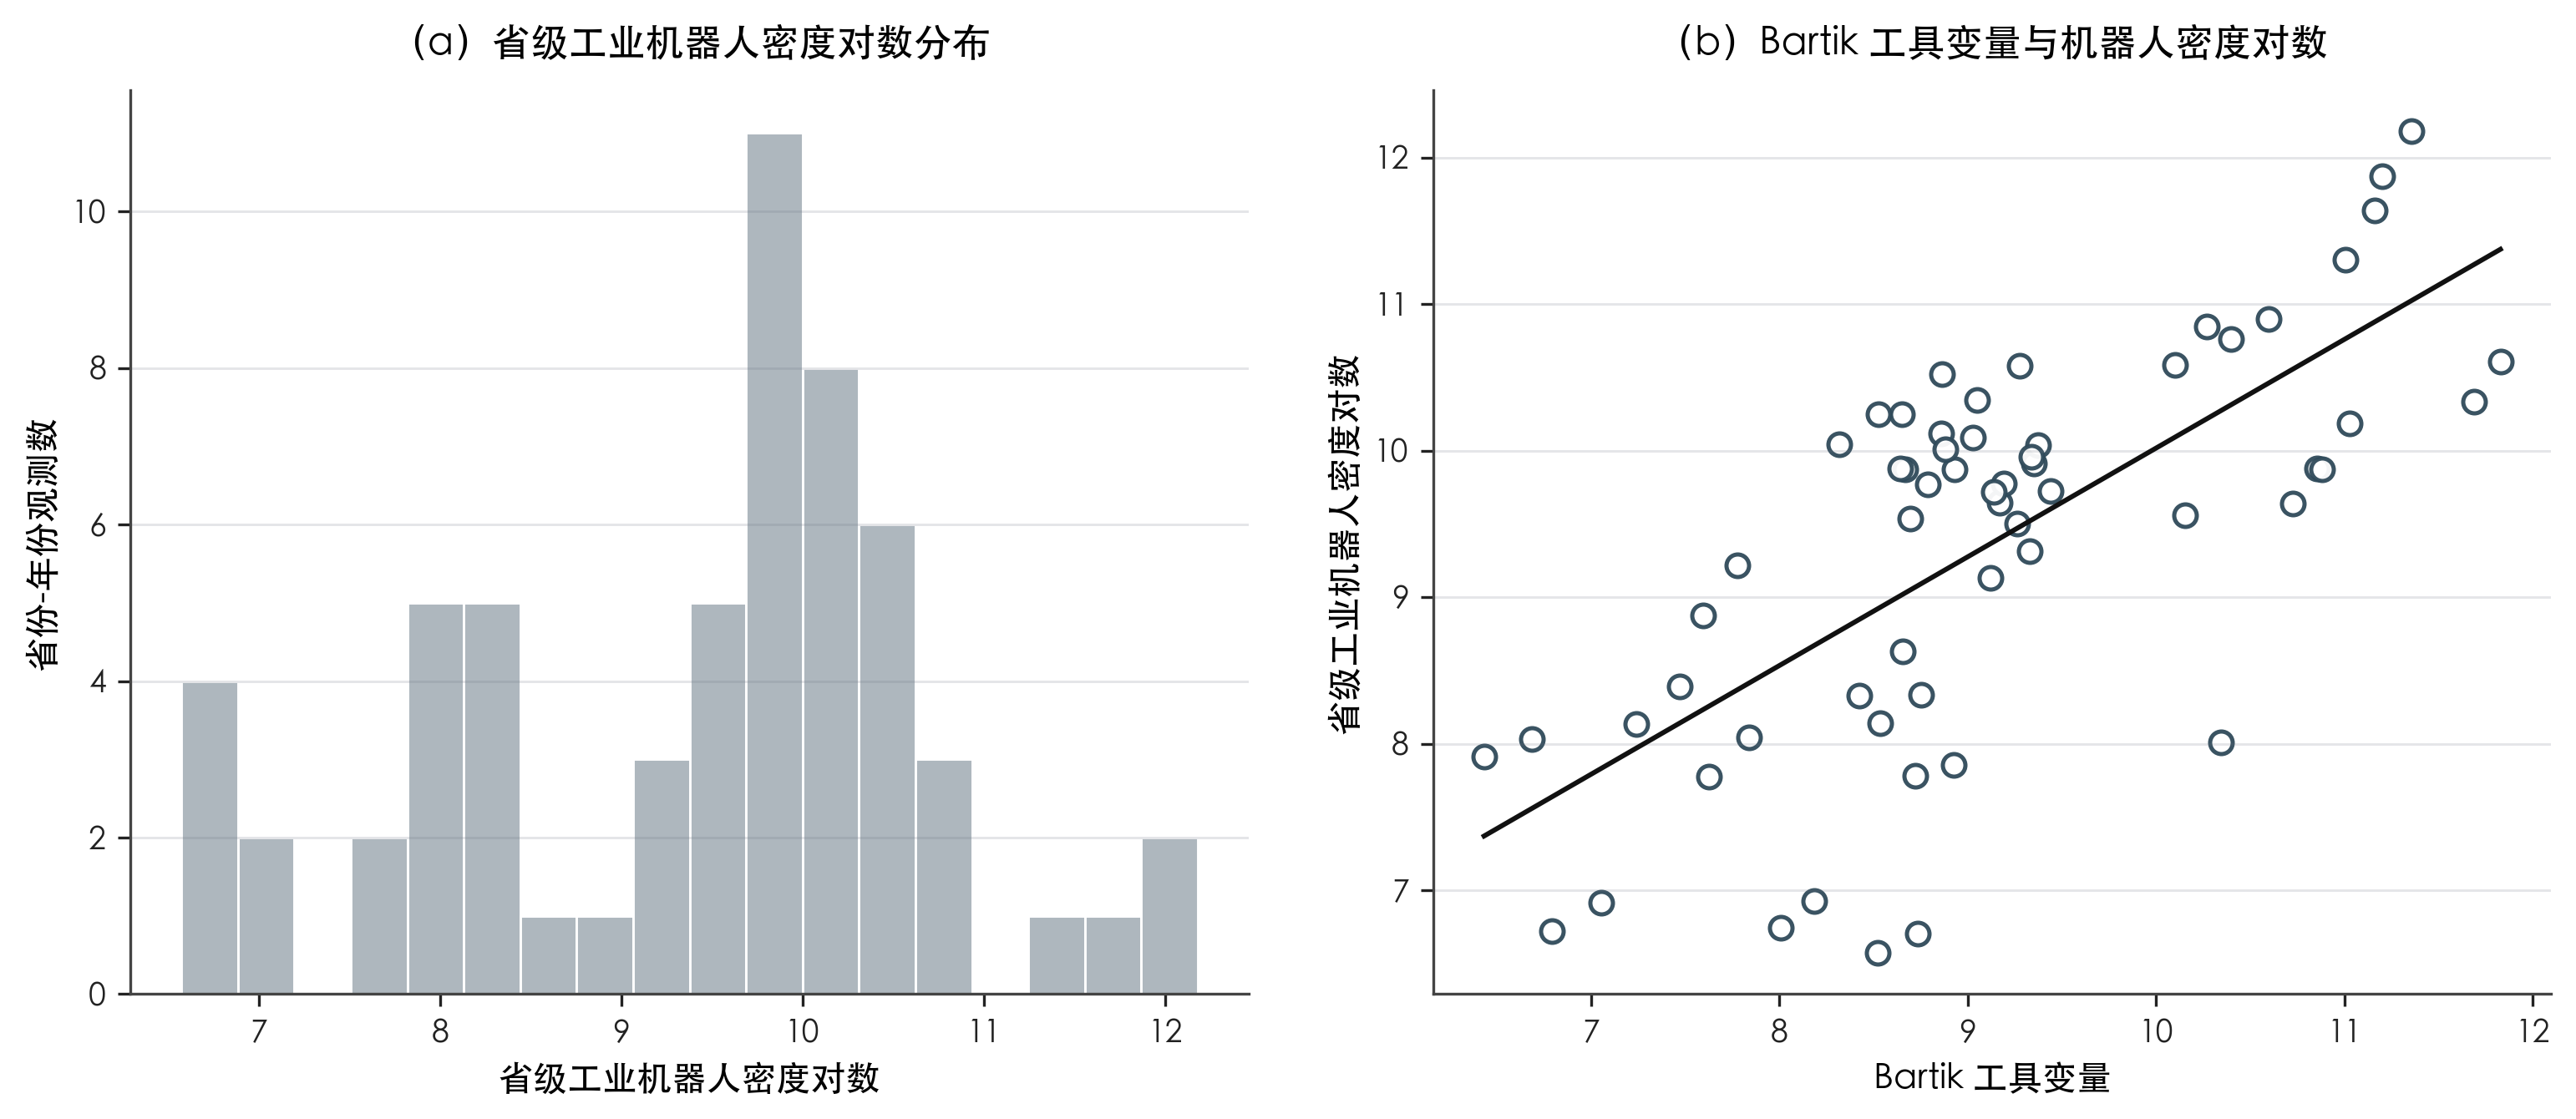
\includegraphics[keepaspectratio]{figures/Fig4_1_IV_Distribution.png}}

图4-1 核心变量分布与第一阶段关系

表4-3A和表4-3B报告工具变量相关性和内生性诊断结果。表4-3A按第一阶段回归表形式报告 Bartik 工具变量与机器人密度对数（ln\_robot）的相关性；表4-3B按诊断汇总表形式列出四个因变量有效样本中的第一阶段稳健 F、Partial R² 和 Durbin-Wu-Hausman 内生性检验。两表分别报告第一阶段回归结果和分因变量样本的诊断指标。

\textbf{表4-3A Bartik 工具变量第一阶段回归结果}

{\def\LTcaptype{none} % do not increment counter
\begin{longtable}[]{@{}lr@{}}
\toprule\noalign{}
变量 & (1) 机器人密度对数（ln\_robot） \\
\midrule\noalign{}
\endhead
\bottomrule\noalign{}
\endlastfoot
Bartik 工具变量 & 0.7544*** \\
& (0.1910) \\
\textbf{模型设定} & \\
个体控制变量 & 是 \\
年份固定效应 & 是 \\
聚类层级 & 省份 \\
观测值 & 30,049 \\
R² & 0.480 \\
\end{longtable}
}

数据来源：CFPS 2020、2022，IFR 工业机器人数据及省级产业结构资料。

注：本表报告 Bartik 工具变量预测机器人密度对数（ln\_robot）的第一阶段回归。回归控制年龄、性别、受教育程度、城乡属性和年份固定效应；括号内为按省份聚类的稳健标准误。一个星号、两个星号、三个星号分别表示在 10\%、5\% 和 1\% 水平上显著。

\textbf{表4-3B 分因变量样本的工具变量诊断}

{\def\LTcaptype{none} % do not increment counter
\begin{longtable}[]{@{}lrrrr@{}}
\toprule\noalign{}
诊断项 & 工资对数 & 制造业就业 & ISEI 得分 & 兼职就业 \\
\midrule\noalign{}
\endhead
\bottomrule\noalign{}
\endlastfoot
有效样本量 N & 15,697 & 18,231 & 28,974 & 28,646 \\
第一阶段稳健 F & 14.03 & 14.29 & 15.55 & 15.38 \\
Partial R² & 0.4834 & 0.4896 & 0.4573 & 0.4553 \\
DWH F 统计量 & 14.27 & 11.28 & 8.19 & 15.60 \\
DWH p 值 & 0.0007 & 0.0022 & 0.0077 & 0.0005 \\
\end{longtable}
}

数据来源：CFPS 2020、2022，IFR 工业机器人数据及省级产业结构资料。

注：各列对应不同因变量进入 IV 估计和诊断检验时的有效样本。第一阶段稳健 F、Partial R² 和 Durbin-Wu-Hausman 检验结果来自相同有效样本；DWH 检验的原假设为机器人密度对数外生。Stock-Yogo 临界值在省级聚类稳健标准误下仅作补充参照。

基准模型用于估计省级机器人暴露与个体劳动力市场配置结果之间的关系；CLDS 补充模型则用于观察岗位适配和求职调整相关变量。

\subsection{CLDS 补充分析模型}\label{clds-ux8865ux5145ux5206ux6790ux6a21ux578b}

CLDS 补充分析用于考察省级机器人暴露与岗位适配、技能吸收和求职行为之间的经验关联。

本文使用 CLDS 2016 和 CLDS 2018 合并重复截面样本，保留 16---60 岁且能匹配机器人暴露和核心控制变量的劳动者。补充分析模型设定为：

\[
M_{ipt}=\delta_0+\delta_1RobotExposure_{pt}+\delta_2X_{ipt}+\tau_t+\nu_{ipt}
\]

其中，\(i\) 表示个体，\(p\) 表示省份，\(t\) 表示调查年份。CLDS 补充分析中的被解释变量记为 \(M_{ipt}\)，依次包括是否找过工作（searched\_recent）、找工作时间（月字段）（search\_months）、当前岗位是否需要培训（need\_training）、掌握岗位技能所需时间类别（skill\_time）、是否参加技术培训（tech\_training）以及证书---岗位不匹配（cert\_mismatch）。这些变量分别对应求职状态和找工作时间（月字段）、岗位培训要求、技能吸收过程和资格适配关系。

省份---年份层面的机器人暴露强度记为 \(RobotExposure_{pt}\)，在 CLDS 补充分析模型中使用省级机器人密度对数的标准化形式；该标准化在合并分析样本中完成。CLDS 2016 年和 2018 年样本分别匹配同年省级机器人暴露。个体控制变量记为 \(X_{ipt}\)，包括年龄、性别和受教育程度；年份固定效应记为 \(\tau_t\)，用于控制 2016 年和 2018 年之间共同的时间变化。为处理同一省份内个体误差项可能相关的问题，本文在 CLDS 补充分析回归中将标准误按省份层面聚类。

CLDS 样本为重复截面数据，且该模型未使用 Bartik 工具变量。二元变量按线性概率模型解释，掌握岗位技能所需时间类别按原始有序时间类别进行线性处理，找工作时间（月字段）仅保留求职时间题项中的月数字段，证书---岗位不匹配仅在持有职业证书的样本中解释。因此，\(\delta_1\) 表示控制年龄、性别、受教育程度和年份固定效应后，省级机器人密度对数提高 1 个标准差时，CLDS 调整过程变量的平均差异。

第 5 章先报告 CFPS 基准估计结果，再在 CLDS 补充分析部分呈现调整过程分析结果。

\chapter{实证结果分析}\label{ux5b9eux8bc1ux7ed3ux679cux5206ux6790}

\section{基准回归结果分析}\label{ux57faux51c6ux56deux5f52ux7ed3ux679cux5206ux6790}

本节报告基于 CFPS 个体样本和 Bartik 工具变量的两阶段估计结果。表5-1报告工资对数、制造业就业、ISEI 得分和兼职就业四项配置结果的 IV-2SLS 基准估计；表5-2保留工资和制造业就业两个核心结果，比较普通最小二乘估计、简化式估计和工具变量两阶段估计下的方向。

表5-1报告机器人暴露与劳动者配置结果之间的 IV-2SLS 基准关系。系数方向上，工资对数、制造业就业和 ISEI 得分三列为正，兼职就业列为负。显著性上，工资方程中机器人密度对数的估计系数为 0.1994，标准误为 0.0780，在 5\% 水平上显著；制造业就业方程的系数为 0.0798，在 1\% 水平上显著；ISEI 得分方程的系数为 0.9995，在 1\% 水平上显著；兼职就业方程的系数为 -0.0162，在 10\% 水平上显著，统计证据弱于前三类结果。

从经济含义看，工具变量预测的省级机器人密度对数提高 1 个单位，与工资对数上升约 0.1994、制造业就业概率提高约 7.98 个百分点相对应；ISEI 得分系数表示职业社会经济地位得分提高约 1 分。兼职就业为二元变量，系数为 -0.0162，表示兼职就业概率下降约 1.62 个百分点，但该结果只在 10\% 水平上显著。表5-1中，工资回报、制造业就业和职业层级构成本文主要配置结果；兼职就业反映工作时间安排，后文结合稳健性检验和年龄组结果继续讨论。

\textbf{表5-1 工业机器人暴露与劳动者配置结果：IV-2SLS 基准估计}

{\def\LTcaptype{none} % do not increment counter
\begin{longtable}[]{@{}lrrrr@{}}
\toprule\noalign{}
变量 & (1) 工资对数 & (2) 制造业就业 & (3) ISEI 得分 & (4) 兼职就业 \\
\midrule\noalign{}
\endhead
\bottomrule\noalign{}
\endlastfoot
机器人密度对数 & 0.1994** & 0.0798*** & 0.9995*** & -0.0162* \\
& (0.0780) & (0.0219) & (0.2746) & (0.0094) \\
\textbf{模型设定} & & & & \\
个体控制变量 & 是 & 是 & 是 & 是 \\
年份固定效应 & 是 & 是 & 是 & 是 \\
省份聚类标准误 & 是 & 是 & 是 & 是 \\
观测值 & 15,697 & 18,231 & 28,974 & 28,646 \\
R² & 0.191 & 0.035 & 0.440 & 0.083 \\
第一阶段稳健 F & 14.03 & 14.29 & 15.55 & 15.38 \\
DWH 检验 p 值 & 0.0007 & 0.0022 & 0.0077 & 0.0005 \\
\end{longtable}
}

数据来源：CFPS 2020、2022，IFR 工业机器人数据及省级产业结构资料。

注：本表报告基于 CFPS 个体样本的 IV-2SLS 估计结果。核心解释变量为省级工业机器人密度对数，工具变量口径见表4-1和4.3.2节。各列均控制年龄、性别、受教育程度、城乡属性和年份固定效应；括号内为按省份聚类的稳健标准误。第一阶段稳健 F 和 DWH 检验 p 值对应各列有效样本，DWH 检验的原假设为机器人密度对数外生。四列因变量量纲不同，系数不作跨列大小比较。一个星号、两个星号、三个星号分别表示在 10\%、5\% 和 1\% 水平上显著。

图5-1a至图5-1d分别展示表5-1中四个结果变量的核心系数及其置信区间，用于观察机器人暴露与不同劳动者配置结果之间的估计方向和统计不确定性。

{\def\LTcaptype{none} % do not increment counter
\begin{longtable}[]{@{}
  >{\raggedright\arraybackslash}p{(\linewidth - 2\tabcolsep) * \real{0.5000}}
  >{\raggedright\arraybackslash}p{(\linewidth - 2\tabcolsep) * \real{0.5000}}@{}}
\toprule\noalign{}
\endhead
\bottomrule\noalign{}
\endlastfoot
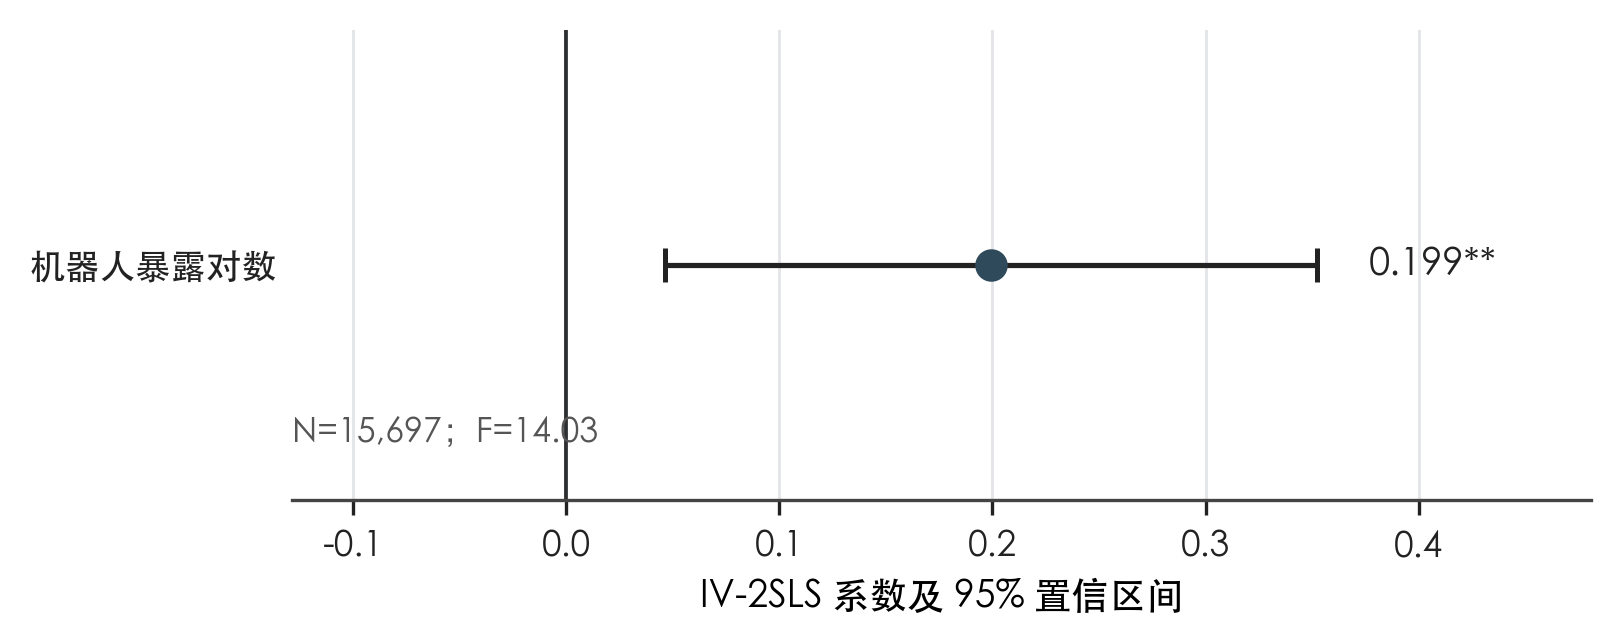
\includegraphics[width=2.75in,height=\textheight,keepaspectratio]{figures/Fig5_1a_Wage_IV_Coefficient.png}图5-1a 工资对数：工具变量估计系数 & 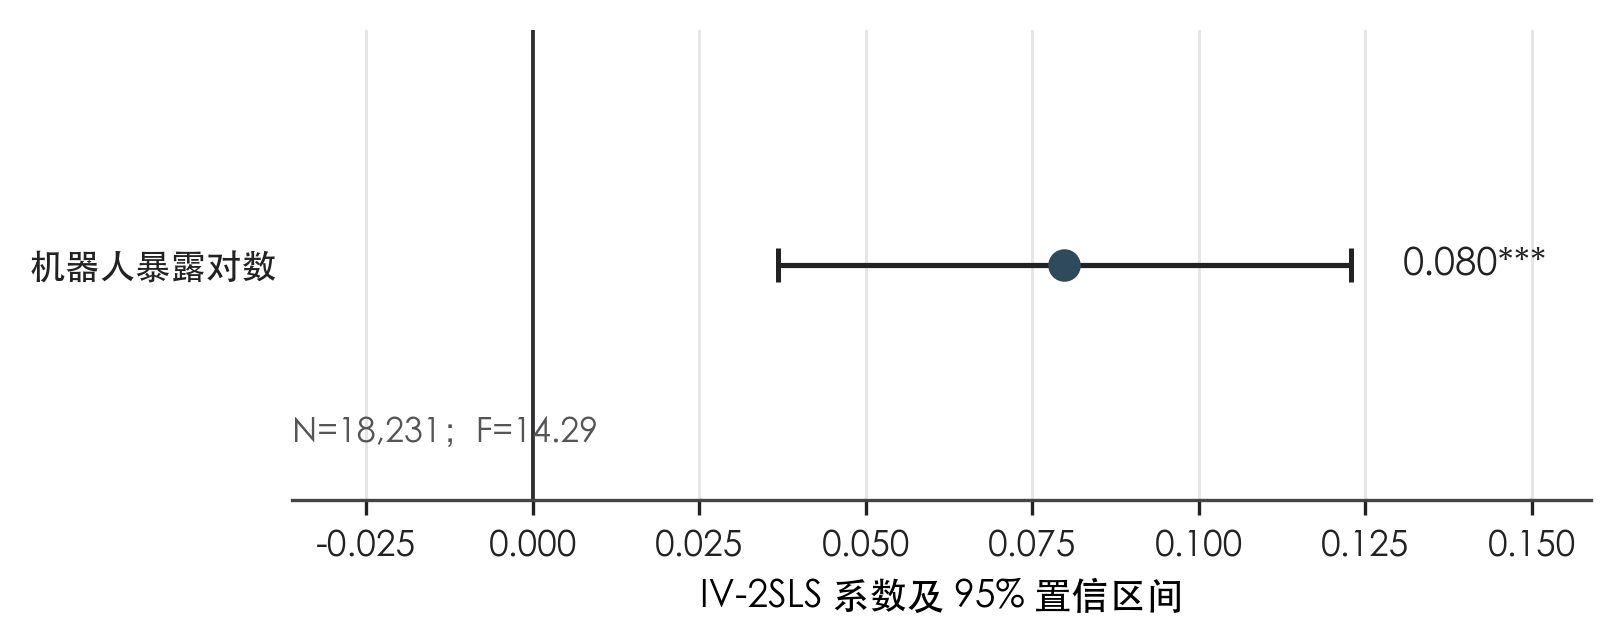
\includegraphics[width=2.75in,height=\textheight,keepaspectratio]{figures/Fig5_1b_Manufacturing_IV_Coefficient.png}图5-1b 制造业就业：工具变量估计系数 \\
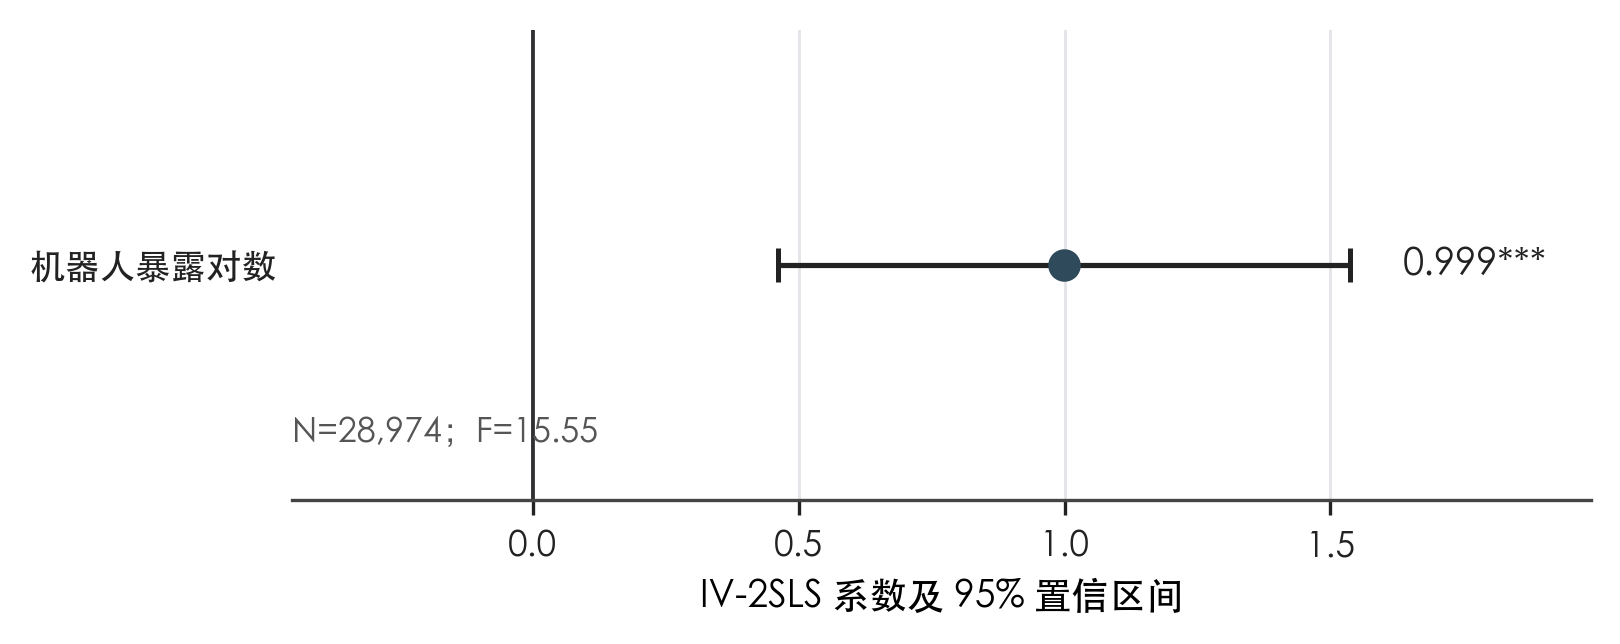
\includegraphics[width=2.75in,height=\textheight,keepaspectratio]{figures/Fig5_1c_ISEI_IV_Coefficient.png}图5-1c ISEI 得分：工具变量估计系数 & 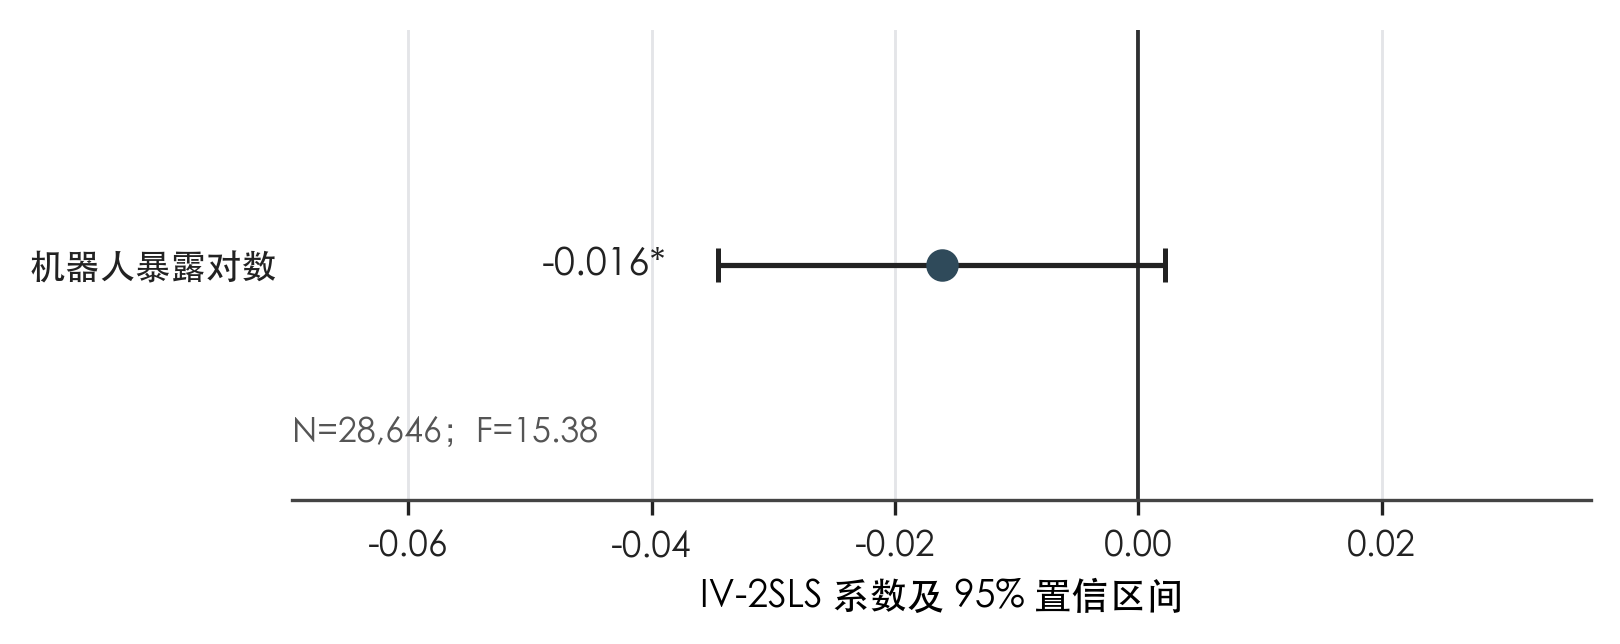
\includegraphics[width=2.75in,height=\textheight,keepaspectratio]{figures/Fig5_1d_PartTime_IV_Coefficient.png}图5-1d 兼职就业：工具变量估计系数 \\
\end{longtable}
}

表5-2进一步比较 OLS、Reduced Form 和 IV-2SLS 三种估计口径下的工资对数和制造业就业结果。OLS 和 IV-2SLS 使用机器人密度对数，Reduced Form 使用 Bartik 工具变量本身，因此该表主要用于核对方向和显著性是否一致，不用于直接比较三类系数大小。

\textbf{表5-2 工资与制造业就业核心结果的不同估计口径比较}

{\def\LTcaptype{none} % do not increment counter
\begin{longtable}[]{@{}lrrr@{}}
\toprule\noalign{}
项目 & (1) OLS & (2) Reduced Form & (3) IV-2SLS \\
\midrule\noalign{}
\endhead
\bottomrule\noalign{}
\endlastfoot
\textbf{Panel A：工资对数} & & & \\
核心解释变量 & 机器人密度对数 & Bartik 工具变量 & 机器人密度对数 \\
系数 & 0.0975*** & 0.1400*** & 0.1994** \\
& (0.0178) & (0.0246) & (0.0780) \\
观测值 & 15,697 & 15,697 & 15,697 \\
R² & 0.207 & 0.221 & 0.192 \\
第一阶段稳健 F & --- & --- & 14.03 \\
DWH 检验 p 值 & --- & --- & 0.0007 \\
\textbf{Panel B：制造业就业} & & & \\
核心解释变量 & 机器人密度对数 & Bartik 工具变量 & 机器人密度对数 \\
系数 & 0.0576*** & 0.0567*** & 0.0798*** \\
& (0.0100) & (0.0107) & (0.0219) \\
观测值 & 18,231 & 18,231 & 18,231 \\
R² & 0.040 & 0.038 & 0.036 \\
第一阶段稳健 F & --- & --- & 14.29 \\
DWH 检验 p 值 & --- & --- & 0.0022 \\
\textbf{模型设定} & & & \\
个体控制变量 & 是 & 是 & 是 \\
年份固定效应 & 是 & 是 & 是 \\
聚类层级 & 省份 & 省份 & 省份 \\
\end{longtable}
}

数据来源：CFPS 2020、2022，IFR 工业机器人数据及省级产业结构资料。

注：OLS 为普通最小二乘估计，IV-2SLS 为工具变量两阶段估计，二者均使用省级机器人密度对数；Reduced Form 使用 Bartik 工具变量作为核心解释变量。三类估计口径的核心解释变量不同，系数不作直接大小比较。第一阶段稳健 F 和 DWH 检验 p 值仅对应 IV-2SLS 估计；``---''表示不适用于对应估计口径。一个星号、两个星号、三个星号分别表示在 10\%、5\% 和 1\% 水平上显著。

表5-2显示，工资方程和制造业就业方程在三种估计口径下均保持正向，说明两项核心结果在不同估计口径下方向一致。完整第一阶段和内生性诊断见表4-3。

图5-2a和图5-2b分别展示工资方程和制造业就业方程在普通最小二乘估计、简化式估计和工具变量两阶段估计下的核心系数及其置信区间。

\pandocbounded{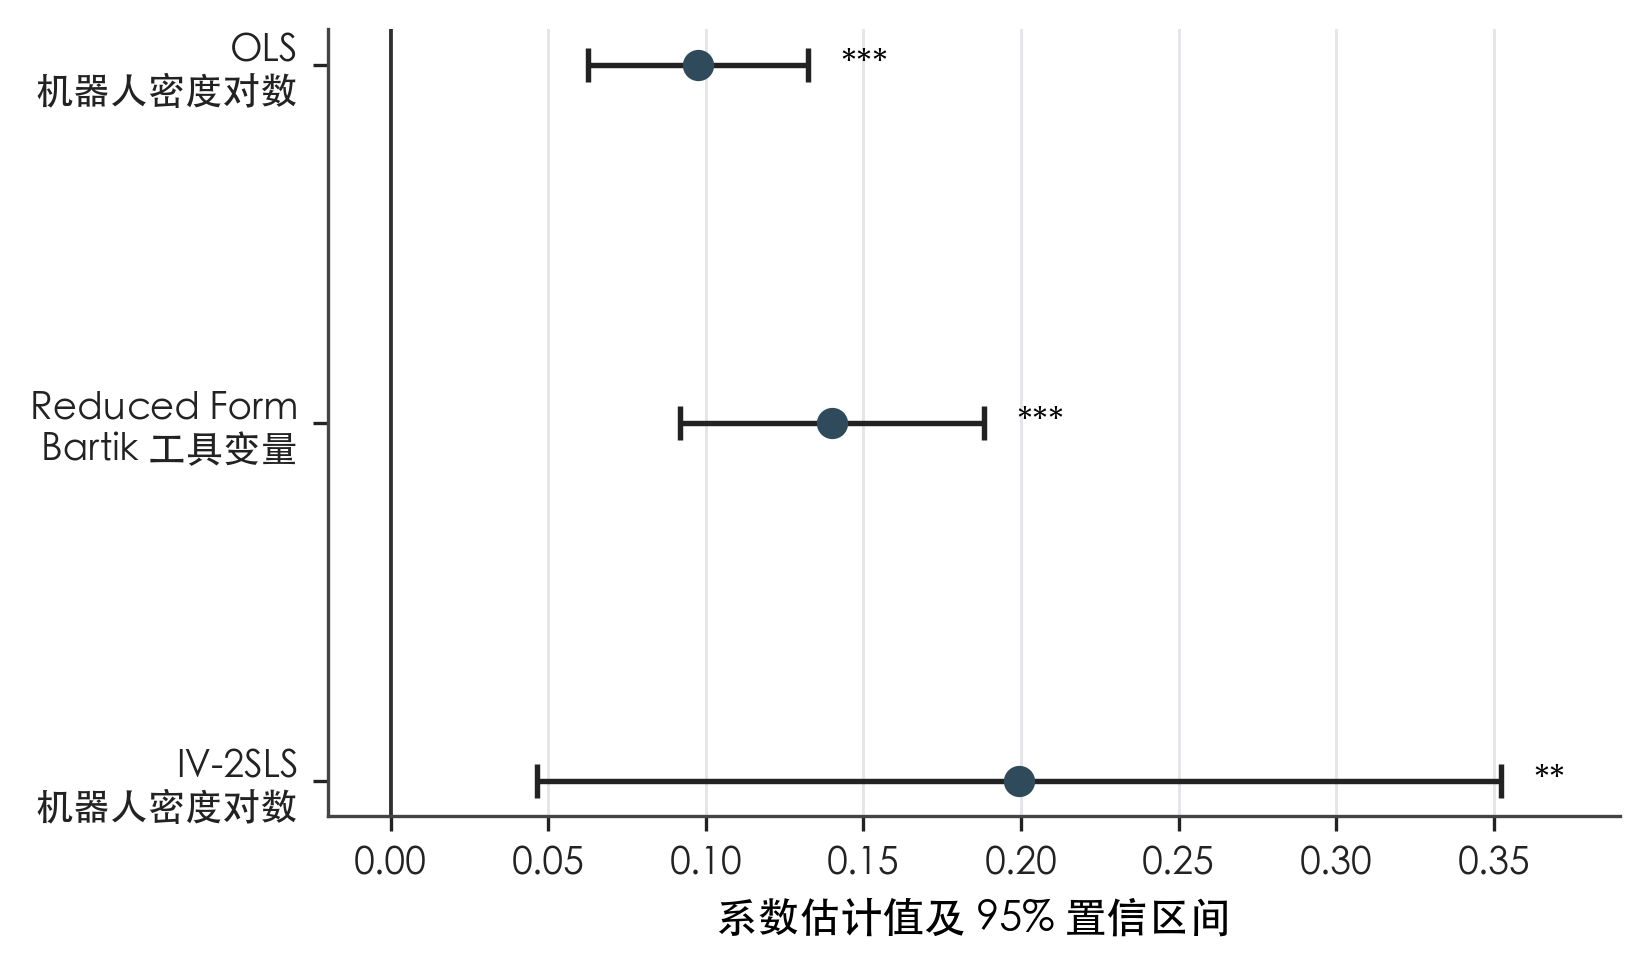
\includegraphics[keepaspectratio]{figures/Fig5_2a_Wage_OLS_RF_IV.png}}

图5-2a 工资方程：不同估计口径下的核心系数比较

\pandocbounded{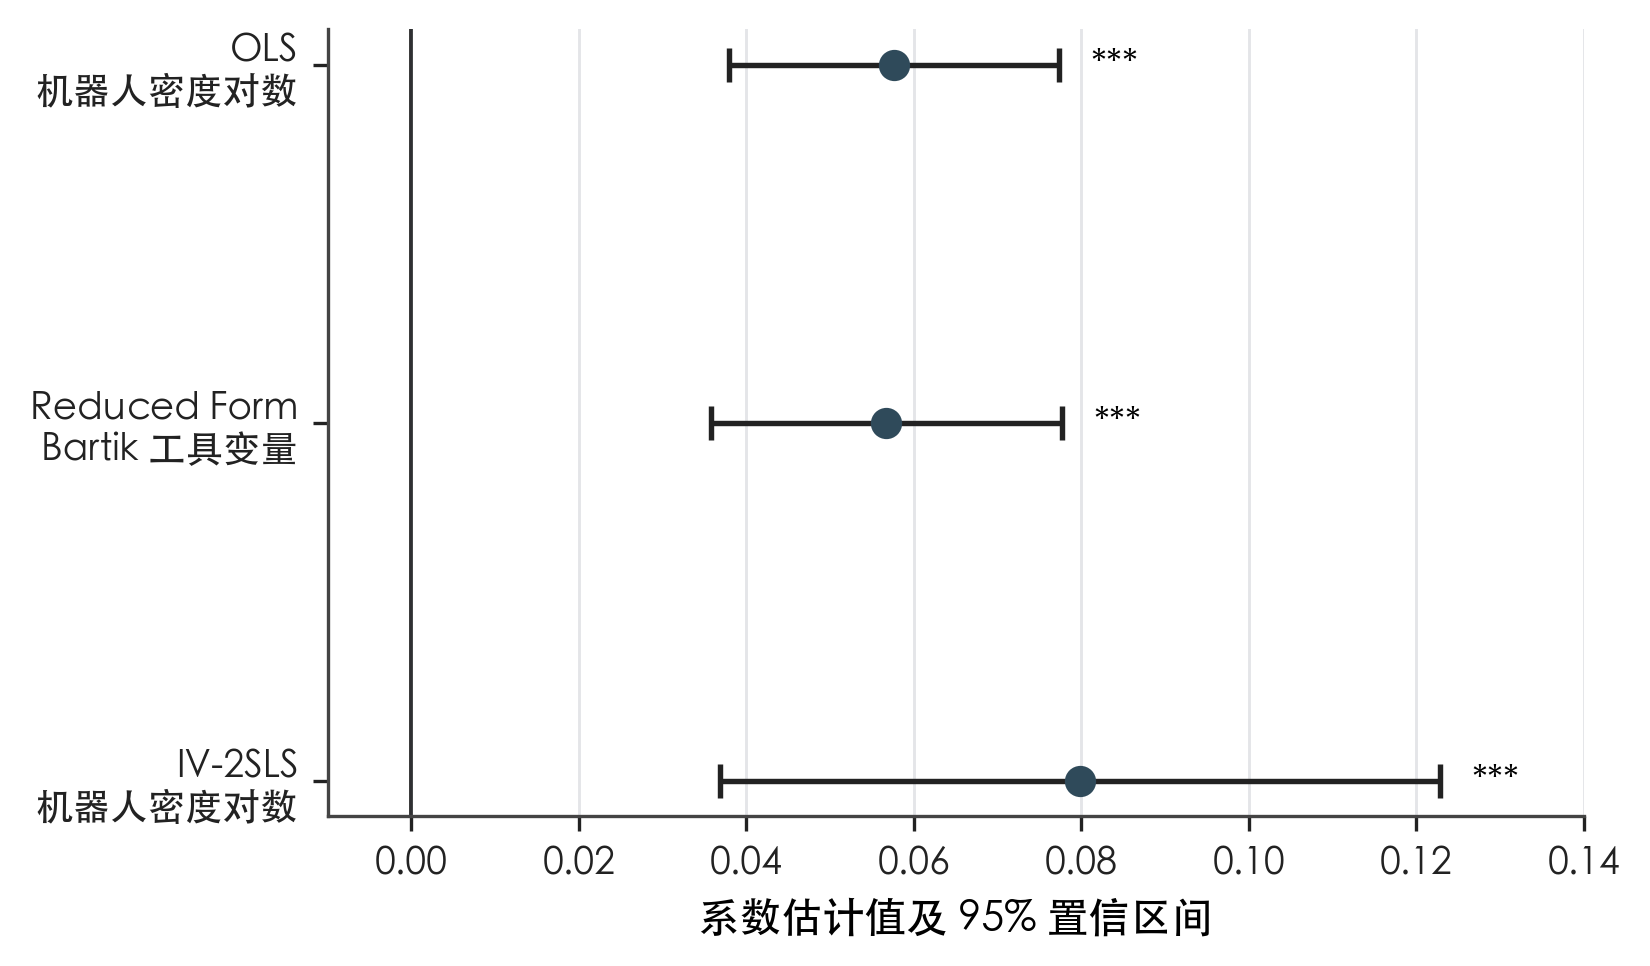
\includegraphics[keepaspectratio]{figures/Fig5_2b_Manufacturing_OLS_RF_IV.png}}

图5-2b 制造业就业方程：不同估计口径下的核心系数比较

综上，在 CFPS 与 Bartik 工具变量设定下，表5-1给出第5章主结果，表5-2说明工资和制造业就业两项核心结果在不同估计口径下方向一致。机器人暴露更高地区的劳动者在工资回报、制造业就业和职业层级上呈现较一致的正向差异。该结果构成本文讨论``劳动者重新配置''的经验基础，下一节将从样本处理、异常值处理、特殊地区排除和变量口径等方面检验其稳定性。

\section{稳健性检验与扩展估计}\label{ux7a33ux5065ux6027ux68c0ux9a8cux4e0eux6269ux5c55ux4f30ux8ba1}

\subsection{样本处理与变量口径稳健性检验}\label{ux6837ux672cux5904ux7406ux4e0eux53d8ux91cfux53e3ux5f84ux7a33ux5065ux6027ux68c0ux9a8c}

基准估计中，工资回报、制造业就业和职业层级结果较清晰，兼职就业结果的统计证据较弱。本节从三个方面检验这些结果的稳定性：剔除 55 岁及以上样本，用于处理临近退休群体的行为差异；对关键变量实施 1\% 缩尾，用于减弱极端值影响；剔除直辖市样本，用于观察结果是否主要受特殊地区驱动。随后，本文补充检验工资和行业配置结果是否依赖单一变量定义。

表5-3报告三类常规处理后的 IV-2SLS 估计结果，并将四类结果变量分别放入四个 Panel。总体来看，工资对数、制造业就业和 ISEI 得分在不同处理下均保持正向且显著，兼职就业结果相对不稳定。工资方程在剔除 55 岁及以上样本、1\% 缩尾和剔除直辖市后，估计系数分别为 0.2008、0.1915 和 0.1254，均达到常规显著水平；制造业就业的估计系数在 0.0746 至 0.0805 之间，ISEI 得分也保持正向显著。相比之下，兼职就业在剔除直辖市后不再显著，说明工作状态结果的稳定性弱于工资、制造业就业和职业层级结果。

\textbf{表5-3 工业机器人应用对配置结果的常规稳健性检验：IV-2SLS 估计}

{\def\LTcaptype{none} % do not increment counter
\begin{longtable}[]{@{}
  >{\raggedright\arraybackslash}p{(\linewidth - 8\tabcolsep) * \real{0.2000}}
  >{\raggedleft\arraybackslash}p{(\linewidth - 8\tabcolsep) * \real{0.2000}}
  >{\raggedleft\arraybackslash}p{(\linewidth - 8\tabcolsep) * \real{0.2000}}
  >{\raggedleft\arraybackslash}p{(\linewidth - 8\tabcolsep) * \real{0.2000}}
  >{\raggedleft\arraybackslash}p{(\linewidth - 8\tabcolsep) * \real{0.2000}}@{}}
\toprule\noalign{}
\begin{minipage}[b]{\linewidth}\raggedright
结果变量 / 指标
\end{minipage} & \begin{minipage}[b]{\linewidth}\raggedleft
基准估计
\end{minipage} & \begin{minipage}[b]{\linewidth}\raggedleft
剔除 55 岁及以上样本
\end{minipage} & \begin{minipage}[b]{\linewidth}\raggedleft
1\% 缩尾处理
\end{minipage} & \begin{minipage}[b]{\linewidth}\raggedleft
剔除直辖市
\end{minipage} \\
\midrule\noalign{}
\endhead
\bottomrule\noalign{}
\endlastfoot
\textbf{Panel A：工资对数} & & & & \\
机器人密度对数 & 0.1994** & 0.2008*** & 0.1915*** & 0.1254*** \\
& (0.0780) & (0.0759) & (0.0742) & (0.0229) \\
观测值 & 15,697 & 13,846 & 15,697 & 14,232 \\
\textbf{Panel B：制造业就业} & & & & \\
机器人密度对数 & 0.0798*** & 0.0805*** & 0.0798*** & 0.0746*** \\
& (0.0219) & (0.0208) & (0.0219) & (0.0217) \\
观测值 & 18,231 & 16,129 & 18,231 & 16,622 \\
\textbf{Panel C：ISEI 得分} & & & & \\
机器人密度对数 & 0.9995*** & 1.0006*** & 0.9995*** & 0.7905*** \\
& (0.2746) & (0.2354) & (0.2746) & (0.1849) \\
观测值 & 28,974 & 21,895 & 28,974 & 27,199 \\
\textbf{Panel D：兼职就业} & & & & \\
机器人密度对数 & -0.0162* & -0.0168** & -0.0162* & -0.0120 \\
& (0.0094) & (0.0077) & (0.0094) & (0.0077) \\
观测值 & 28,646 & 21,705 & 28,646 & 26,874 \\
\textbf{模型设定} & & & & \\
个体控制变量 & 是 & 是 & 是 & 是 \\
年份固定效应 & 是 & 是 & 是 & 是 \\
聚类层级 & 省份 & 省份 & 省份 & 省份 \\
\end{longtable}
}

数据来源：CFPS 2020、2022，IFR 工业机器人数据及省级产业结构资料。

注：本表报告不同稳健性处理下省级机器人密度对数的 IV-2SLS 估计系数，工具变量口径见表4-1和4.3.2节。各列控制年龄、性别、受教育程度、城乡属性和年份固定效应；括号内为按省份聚类的稳健标准误。1\% 缩尾处理针对工资对数和年龄变量；剔除直辖市指剔除北京、天津、上海和重庆。基准列的第一阶段和内生性诊断见表4-3。一个星号、两个星号、三个星号分别表示在 10\%、5\% 和 1\% 水平上显著。

在样本处理检验之外，本文进一步围绕工资回报和行业配置两个核心结果进行补充口径检验。表5-3a显示，将工资变量替换为按年工作收入和每周工作时间折算的小时收入代理后，机器人密度对数系数仍为正，并在 5\% 水平上显著；将行业结果替换为服务业就业虚拟变量后，机器人密度对数系数为负，并在 5\% 水平上显著。该结果与表5-1中工资回报和制造业就业的方向一致，表明两项核心结果在替代收入口径和行业归类口径下仍具有一定稳定性。

\textbf{表5-3a 工资与行业配置结果的替代变量口径检验}

{\def\LTcaptype{none} % do not increment counter
\begin{longtable}[]{@{}
  >{\raggedright\arraybackslash}p{(\linewidth - 10\tabcolsep) * \real{0.1667}}
  >{\raggedright\arraybackslash}p{(\linewidth - 10\tabcolsep) * \real{0.1667}}
  >{\raggedleft\arraybackslash}p{(\linewidth - 10\tabcolsep) * \real{0.1667}}
  >{\raggedleft\arraybackslash}p{(\linewidth - 10\tabcolsep) * \real{0.1667}}
  >{\raggedleft\arraybackslash}p{(\linewidth - 10\tabcolsep) * \real{0.1667}}
  >{\raggedleft\arraybackslash}p{(\linewidth - 10\tabcolsep) * \real{0.1667}}@{}}
\toprule\noalign{}
\begin{minipage}[b]{\linewidth}\raggedright
结果变量
\end{minipage} & \begin{minipage}[b]{\linewidth}\raggedright
变量口径
\end{minipage} & \begin{minipage}[b]{\linewidth}\raggedleft
系数
\end{minipage} & \begin{minipage}[b]{\linewidth}\raggedleft
标准误
\end{minipage} & \begin{minipage}[b]{\linewidth}\raggedleft
观测值
\end{minipage} & \begin{minipage}[b]{\linewidth}\raggedleft
第一阶段稳健 F
\end{minipage} \\
\midrule\noalign{}
\endhead
\bottomrule\noalign{}
\endlastfoot
小时收入代理 & 年工作收入除以每周工作时间和 52 周后取对数 & 0.2176** & 0.0864 & 15,514 & 13.96 \\
服务业就业 & 当前主要工作行业属于服务业 & -0.0328** & 0.0138 & 18,231 & 14.29 \\
\end{longtable}
}

数据来源：CFPS 2020、2022，IFR 工业机器人数据及省级产业结构资料。

注：本表报告替代被解释变量口径下省级机器人密度对数的 IV-2SLS 估计系数，工具变量口径与表5-1一致。小时收入代理由个人问卷工作总收入与每周工作时间折算得到；服务业就业虚拟变量依据当前主要工作行业编码构造，取值范围为 6---20。各列控制年龄、性别、受教育程度、城乡属性和年份固定效应；标准误按省份聚类。一个星号、两个星号、三个星号分别表示在 10\%、5\% 和 1\% 水平上显著。

综合表5-3和表5-3a可见，在样本筛选、极端值处理、特殊地区排除以及替代工资和行业口径下，工资回报和制造业就业的主要结论总体保持一致；职业层级结果在常规样本处理下也较为稳定，但其替代口径结果见附录补充诊断；兼职就业在常规稳健性处理中方向一致，但显著性弱于前三类结果。为检验结论是否依赖两期样本窗口，本文进一步考察基准结论在多年份样本中的表现。

\subsection{多年份样本扩展估计}\label{ux591aux5e74ux4efdux6837ux672cux6269ux5c55ux4f30ux8ba1}

表5-4比较两年基准模型和多年份扩展模型，用于观察基准结论在样本年份扩展后的变化。多年份扩展模型使用 CFPS 2014、2016、2018、2020 和 2022 五期个人数据；机器人暴露变量按调查年前一年匹配，主要对应 2013、2015、2017、2019 和 2021 年的省级机器人暴露。工资方程在两年基准模型和多年份扩展模型中的估计系数分别为 0.1994 和 0.1839，制造业就业方程的对应系数分别为 0.0798 和 0.1056，均保持正向且达到常规显著水平。

图5-3展示多年份样本中省级工业机器人密度对数的年度变化。该图以省份---年份为观测层级，报告各调查年份的省份均值和省份四分位区间。2014 至 2022 年间，省级工业机器人密度对数整体上升，说明多年份扩展模型覆盖了机器人暴露持续变化的时间窗口。

\pandocbounded{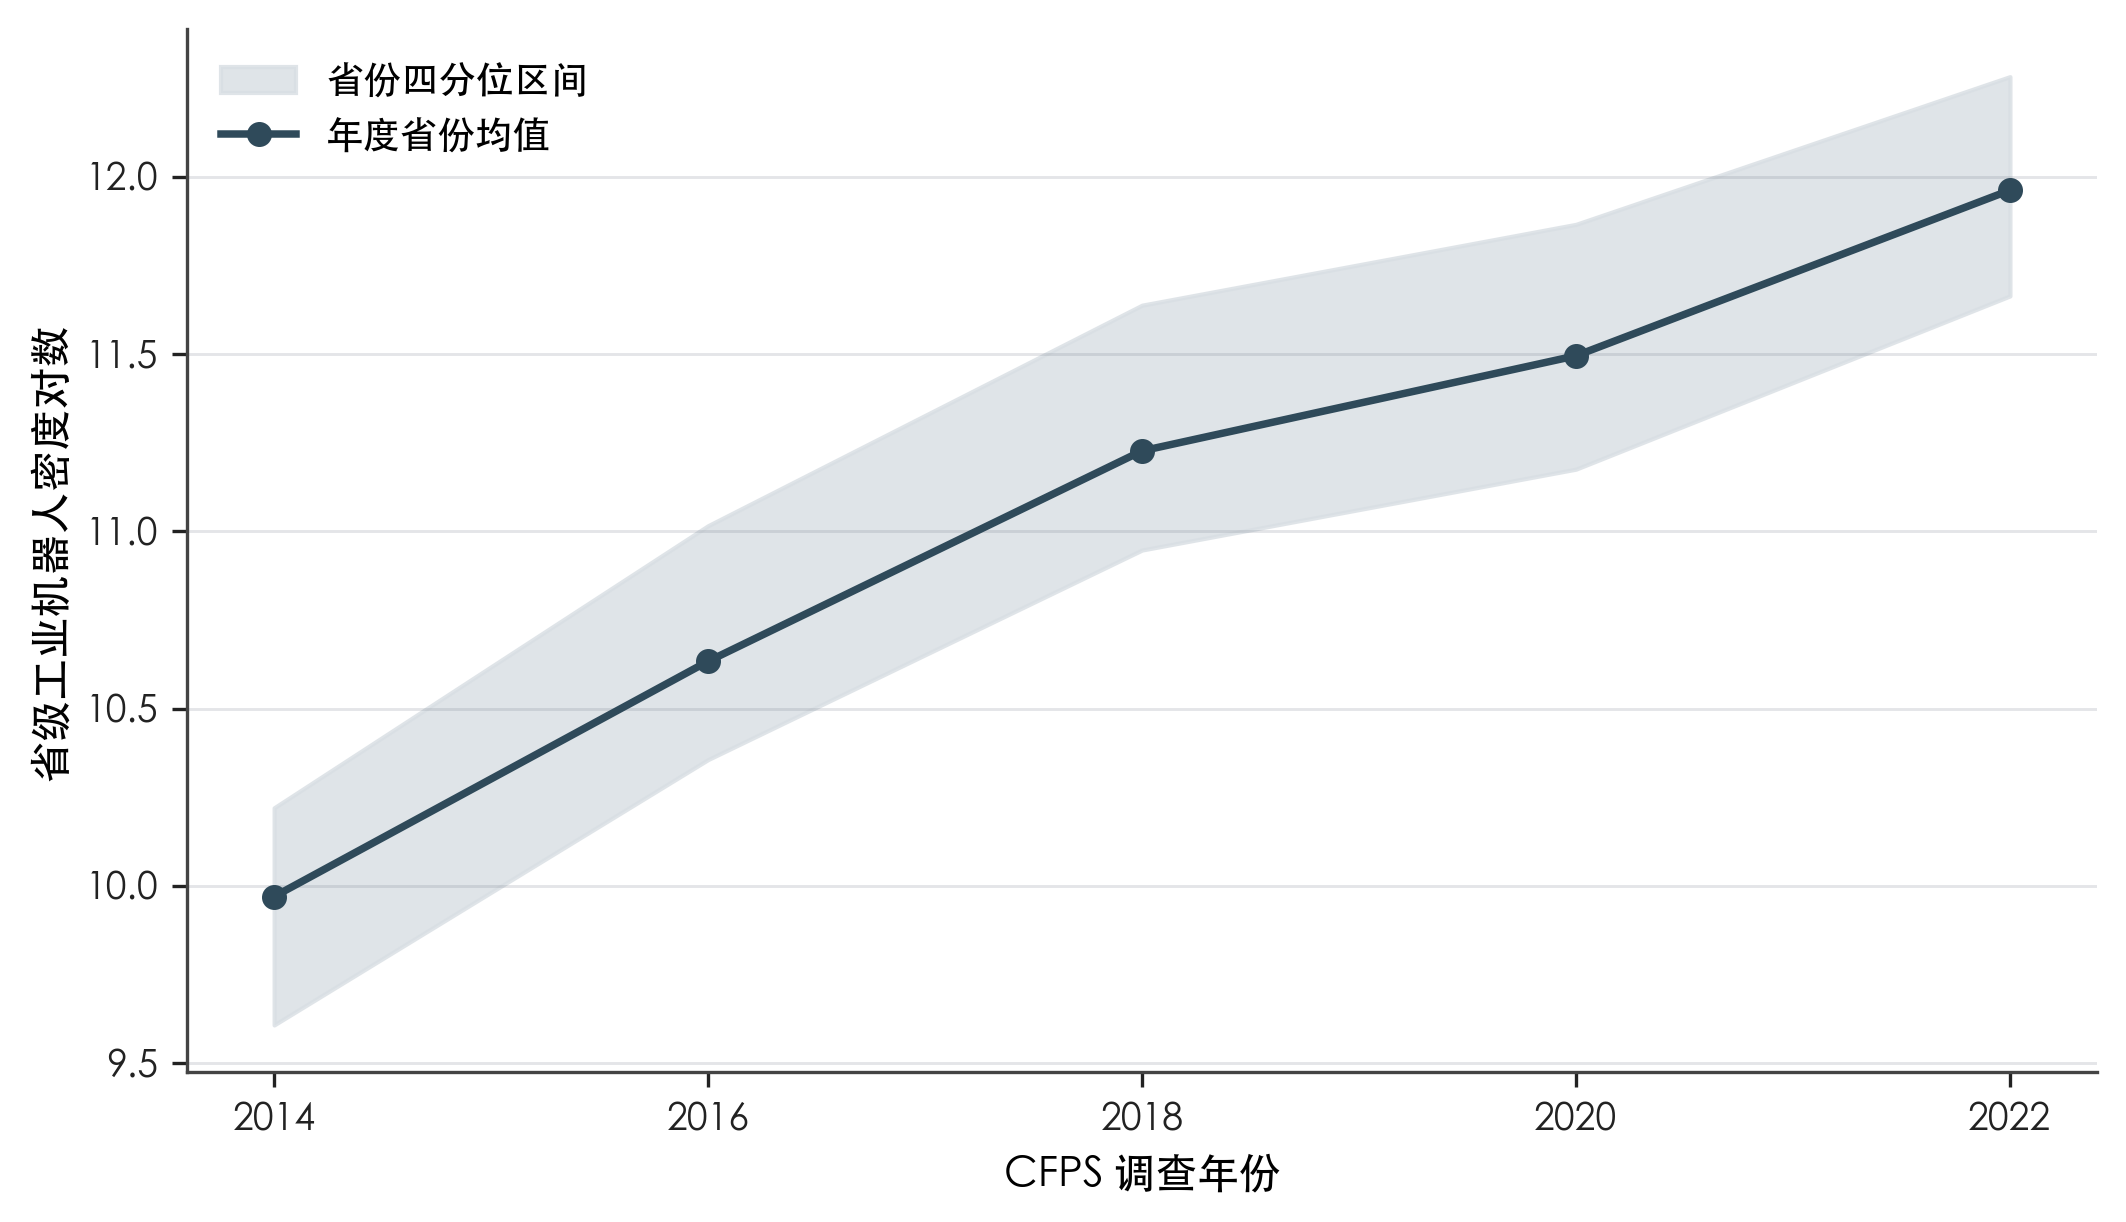
\includegraphics[keepaspectratio]{figures/Fig5_3_Multiwave_Robot_Exposure_Trend.png}}

图5-3 多年份样本中的省级工业机器人密度对数变化

除工资和制造业就业外，表5-4还报告 ISEI 得分和兼职就业结果。ISEI 得分在两年基准模型和多年份扩展模型中均为正向且显著，说明职业层级结果在扩展样本窗口后仍提供同向信息。兼职就业在两年基准模型中为负向且在 10\% 水平上显著，多年份扩展模型中接近于零，表明工作时间安排结果的稳定性弱于工资、行业配置和职业层级结果。

多年份扩展模型扩大了调查年份范围，但仍沿用本文基准模型的控制变量和年份固定效应设定。表5-4因此主要用于说明：在五期 CFPS 样本中，工资、制造业就业和职业层级结果与两年基准估计方向一致；兼职就业结果则对样本窗口更为敏感。

\textbf{表5-4 多年份样本扩展的 IV-2SLS 估计比较}

{\def\LTcaptype{none} % do not increment counter
\begin{longtable}[]{@{}lrr@{}}
\toprule\noalign{}
结果变量 / 指标 & (1) 两年基准 & (2) 多年份扩展 \\
\midrule\noalign{}
\endhead
\bottomrule\noalign{}
\endlastfoot
\textbf{Panel A：工资对数} & & \\
机器人密度对数 & 0.1994** & 0.1839*** \\
& (0.0780) & (0.0602) \\
观测值 & 15,697 & 39,159 \\
\textbf{Panel B：制造业就业} & & \\
机器人密度对数 & 0.0798*** & 0.1056*** \\
& (0.0219) & (0.0197) \\
观测值 & 18,231 & 136,996 \\
\textbf{Panel C：ISEI 得分} & & \\
机器人密度对数 & 0.9995*** & 2.2839*** \\
& (0.2746) & (0.4854) \\
观测值 & 28,974 & 101,116 \\
\textbf{Panel D：兼职就业} & & \\
机器人密度对数 & -0.0162* & 0.0023 \\
& (0.0094) & (0.0282) \\
观测值 & 28,646 & 78,553 \\
\textbf{模型设定} & & \\
样本窗口 & 两期 & 五期 \\
个体控制变量 & 是 & 是 \\
年份固定效应 & 是 & 是 \\
聚类层级 & 省份 & 省份 \\
\end{longtable}
}

数据来源：CFPS 2014、2016、2018、2020、2022，IFR 工业机器人数据及省级产业结构资料。

注：本表报告省级机器人密度对数的 IV-2SLS 估计系数，工具变量口径与表5-1一致。两期指 CFPS 2020 和 2022；五期指 CFPS 2014、2016、2018、2020 和 2022，机器人暴露按调查年前一年匹配。各列均控制年龄、性别、受教育程度、城乡属性和年份固定效应；括号内为按省份聚类的稳健标准误。一个星号、两个星号、三个星号分别表示在 10\%、5\% 和 1\% 水平上显著。

总体来看，在多年份扩展设定下，工资、制造业就业和 ISEI 得分与两年基准结论方向一致，兼职就业结果则不稳定。结合表5-3、表5-3a和表5-4，本文已从样本范围、极端值、特殊地区、变量口径和年份窗口等方面对基准结论进行检验。由于机器人暴露的行业来源会影响结果适用范围，下一部分进一步考察该变量的行业构成。

\section{机器人暴露的行业来源分析}\label{ux673aux5668ux4ebaux66b4ux9732ux7684ux884cux4e1aux6765ux6e90ux5206ux6790}

由于本文机器人暴露变量由行业机器人扩散与省级产业结构共同构造，暴露来源会影响估计结果的经济含义。为此，本文对多年份机器人暴露进行行业来源分解，并进一步实施逐行业剔除检验。

结果显示，制造业贡献了绝大部分机器人暴露，贡献占比约为 99.8\%。在剔除农业、采矿业、公用事业和建筑业后，工资和制造业就业结果仍保持正向；剔除制造业后，相关估计结果发生明显变化。上述结果说明，本文识别到的机器人暴露主要来自制造业机器人扩散，因此本文结论主要对应制造业机器人扩散占主导的经验背景。完整行业来源分解和逐行业剔除结果见附表A。

在完成主结果、稳健性检验和行业来源说明后，本文转向 CLDS 补充分析，观察求职、岗位技能掌握和证书---岗位适配等调整过程变量。

\section{补充分析：岗位适配、求职状态与工作时间安排}\label{ux8865ux5145ux5206ux6790ux5c97ux4f4dux9002ux914dux6c42ux804cux72b6ux6001ux4e0eux5de5ux4f5cux65f6ux95f4ux5b89ux6392}

\subsection{岗位适配与求职状态的 CLDS 补充分析}\label{ux5c97ux4f4dux9002ux914dux4e0eux6c42ux804cux72b6ux6001ux7684-clds-ux8865ux5145ux5206ux6790}

在 CFPS 基准结果之外，本文使用 CLDS 2016 和 2018 合并样本观察求职状态、培训参与、岗位技能掌握和证书---岗位适配等调整过程变量的相关变化。表5-5中的六个变量包括是否需要培训、掌握岗位技能所需时间类别、是否参加技术培训、证书---岗位不匹配、是否找过工作和找工作时间（月字段）。该部分未使用 Bartik 工具变量，主要提供调整过程中的相关关系证据。

\textbf{表5-5 机器人暴露与 CLDS 调整过程变量的相关关系}

{\def\LTcaptype{none} % do not increment counter
\begin{longtable}[]{@{}lrr@{}}
\toprule\noalign{}
调整维度 / 因变量 & 系数（机器人暴露标准化值） & 观测值 \\
\midrule\noalign{}
\endhead
\bottomrule\noalign{}
\endlastfoot
\textbf{Panel A：培训与岗位技能掌握} & & \\
是否需要培训 & -0.0091* & 9,305 \\
& (0.0052) & \\
掌握岗位技能所需时间类别 & -0.1620*** & 8,221 \\
& (0.0297) & \\
是否参加技术培训 & -0.0035 & 30,641 \\
& (0.0050) & \\
\textbf{Panel B：资格适配} & & \\
证书---岗位不匹配 & 0.0199*** & 4,046 \\
& (0.0061) & \\
\textbf{Panel C：求职状态} & & \\
是否找过工作 & 0.0136* & 10,718 \\
& (0.0079) & \\
找工作时间（月字段） & -0.4218 & 676 \\
& (0.3640) & \\
\textbf{模型设定} & & \\
个体控制变量 & 是 & \\
年份固定效应 & 是 & \\
聚类层级 & 省份 & \\
Bartik 工具变量 & 否 & \\
\end{longtable}
}

数据来源：CLDS 2016、2018，IFR 工业机器人数据。

注：本表基于 CLDS 2016 和 2018 合并样本，核心解释变量为省级机器人密度对数的标准化值。估计方法为线性回归或线性概率模型；括号内为按省份聚类的稳健标准误。二元变量按概率差异解释；掌握岗位技能所需时间类别按原始有序时间类别解释；找工作时间（月字段）未将周、年字段统一折算；证书---岗位不匹配仅在持有职业证书的样本中解释。一个星号、两个星号、三个星号分别表示在 10\%、5\% 和 1\% 水平上显著。

表5-5的结果主要集中在资格适配和岗位技能掌握两个变量上。具体而言，证书---岗位不匹配系数为 0.0199，并在 1\% 水平上显著；掌握岗位技能所需时间类别的系数为 -0.1620，并在 1\% 水平上显著。是否找过工作为正，是否需要培训为负，二者均在 10\% 水平上显著；技术培训参与和找工作时间（月字段）未呈现显著变化。由于变量量纲和样本限制不同，本节只比较方向和显著性，不比较系数大小。

从解释上看，证书---岗位不匹配上升提示持证劳动者的资格信号与岗位要求之间可能存在更大偏离。掌握岗位技能所需时间类别较低，反映机器人暴露较高地区在岗位技能掌握时间类别、岗位构成或样本结构上存在差异。正式技术培训参与未呈现显著变化，表5-5中的调整迹象主要体现在资格适配和岗位技能掌握，而不是正式培训参与或找工作时间（月字段）的变化。

\subsection{补充结果整合与工作时间安排的年龄组差异}\label{ux8865ux5145ux7ed3ux679cux6574ux5408ux4e0eux5de5ux4f5cux65f6ux95f4ux5b89ux6392ux7684ux5e74ux9f84ux7ec4ux5deeux5f02}

本节收束第5章的补充证据，并针对兼职就业结果在前文中证据较弱的问题报告年龄组检验。前文结果显示，工资回报和制造业就业是本文最清晰的主结果，职业层级提供同向辅助证据；兼职就业在基准估计中出现负向关系，但统计证据弱于前三类结果，因此需要考察其样本结构。

表5-1中，兼职就业系数为 -0.0162，并在 10\% 水平上显著；表5-4中，兼职就业在多年份扩展样本中接近于零，稳定性弱于工资、制造业就业和职业层级结果。因此，兼职就业作为工作时间安排维度的补充结果处理。表5-6进一步按年龄组考察兼职就业结果，用于说明这一较弱结果是否来自不同年龄组之间的差异。

表5-6使用 CFPS 2020 与 2022 样本，报告兼职结果的年龄分组估计和年龄组交互项检验。Panel A 按年龄组分别估计兼职就业方程，用于观察各年龄组内部的系数方向和显著性；Panel B 在全样本中加入机器人暴露与年龄组虚拟变量交互项，用于检验年龄组之间是否存在统计差异。因变量为是否兼职，估计方法与基准 IV-2SLS 设定一致。

\textbf{表5-6 兼职就业结果的年龄组差异与交互项检验}

Panel A：按年龄组分样本估计

{\def\LTcaptype{none} % do not increment counter
\begin{longtable}[]{@{}
  >{\raggedright\arraybackslash}p{(\linewidth - 8\tabcolsep) * \real{0.1579}}
  >{\raggedleft\arraybackslash}p{(\linewidth - 8\tabcolsep) * \real{0.2105}}
  >{\raggedleft\arraybackslash}p{(\linewidth - 8\tabcolsep) * \real{0.2105}}
  >{\raggedleft\arraybackslash}p{(\linewidth - 8\tabcolsep) * \real{0.2105}}
  >{\raggedleft\arraybackslash}p{(\linewidth - 8\tabcolsep) * \real{0.2105}}@{}}
\toprule\noalign{}
\begin{minipage}[b]{\linewidth}\raggedright
指标
\end{minipage} & \begin{minipage}[b]{\linewidth}\raggedleft
全样本
\end{minipage} & \begin{minipage}[b]{\linewidth}\raggedleft
青年组（≤30岁）
\end{minipage} & \begin{minipage}[b]{\linewidth}\raggedleft
中年组（31---50岁）
\end{minipage} & \begin{minipage}[b]{\linewidth}\raggedleft
大龄组（\textgreater50岁）
\end{minipage} \\
\midrule\noalign{}
\endhead
\bottomrule\noalign{}
\endlastfoot
第二阶段：机器人密度对数 & -0.0162* & -0.0081 & -0.0223** & -0.0137 \\
& (0.0094) & (0.0057) & (0.0089) & (0.0150) \\
观测值 & 28,646 & 4,977 & 13,669 & 10,000 \\
\end{longtable}
}

Panel B：机器人暴露与年龄组交互项估计

{\def\LTcaptype{none} % do not increment counter
\begin{longtable}[]{@{}lrrl@{}}
\toprule\noalign{}
变量 / 检验 & 系数或统计量 & p 值 & 说明 \\
\midrule\noalign{}
\endhead
\bottomrule\noalign{}
\endlastfoot
机器人密度对数 & -0.0174* & 0.074 & 大龄组为参照组 \\
& (0.0097) & & \\
机器人密度对数 × 青年组 & 0.0064*** & 0.005 & 相对大龄组的差异 \\
& (0.0023) & & \\
机器人密度对数 × 中年组 & -0.0005 & 0.747 & 相对大龄组的差异 \\
& (0.0014) & & \\
交互项联合检验 & χ²(2)=73.09 & \textless0.001 & 检验两个交互项联合为零 \\
\end{longtable}
}

数据来源：CFPS 2020、2022，IFR 工业机器人数据及省级产业结构资料。

注：Panel A 为按年龄组分样本的 IV-2SLS 估计；Panel B 为全样本交互项估计，大龄组为参照组。是否兼职按周工作时间低于 35 小时构造。各回归均控制年龄、性别、受教育程度、城乡属性和年份固定效应；括号内为按省份聚类的稳健标准误。一个星号、两个星号、三个星号分别表示在 10\%、5\% 和 1\% 水平上显著。

\textbf{年龄组差异。} 表5-6的 Panel A 显示，在以周工作时间低于 35 小时构造的兼职指标上，全样本结果延续表5-1的负向关系，并在 10\% 水平上显著。分组估计中，31---50岁中年组与机器人暴露呈显著负相关（β=-0.0223，p=0.0125），青年组和大龄组结果未达到常规显著水平。该结果说明兼职就业的负向关系在分样本中并不均匀；年龄组之间的统计差异需要结合 Panel B 的交互项检验判断。

\textbf{机器人暴露与年龄组交互结果。} 表5-6的 Panel B 提供组间差异检验。机器人暴露变量主效应为 -0.0174（p=0.074），对应大龄组参照组；青年组交互项系数为 0.0064（p=0.005），说明青年组的兼职负相关幅度相对大龄组更弱；中年组交互项不显著（p=0.747），说明中年组与大龄组之间未观察到显著差异。交互项联合检验为 χ²(2)=73.09，p\textless0.001，说明年龄组差异需要纳入解释。本文据此讨论工作时间安排结果的年龄组差异，解释范围限于兼职就业这一工作状态指标。

与5.4.1的 CLDS 结果相比，表5-6处理的是另一类补充证据。前者说明岗位适配、掌握岗位技能所需时间类别和求职状态的相关变化，后者说明工作时间安排结果在年龄组之间存在差异。二者共同补充说明劳动者重新配置的过程表现，但证据来源和解释对象不同。

第5章形成了四层证据。第一，CFPS-Bartik 设定下，工资回报和制造业就业构成本文主结果，职业层级提供同向辅助证据。第二，常规稳健性检验和多年份扩展说明主结果在样本处理、变量口径和年份窗口变化后总体保持一致。第三，行业来源分析说明机器人暴露变量主要反映制造业机器人扩散。第四，CLDS 补充分析提供求职状态、岗位技能掌握和证书---岗位适配方面的过程证据，兼职年龄组检验说明工作时间安排结果存在年龄组差异。下一章将这些证据整理为研究结论和政策含义。

\chapter{研究结论、政策建议与研究不足}\label{ux7814ux7a76ux7ed3ux8bbaux653fux7b56ux5efaux8baeux4e0eux7814ux7a76ux4e0dux8db3}

\section{研究结论}\label{ux7814ux7a76ux7ed3ux8bba}

本文考察工业机器人扩散背景下的劳动者配置变化。基于 CFPS 2020 与 2022 两期个体数据、IFR 行业机器人数据和 Bartik 工具变量，本文估计机器人暴露与工资回报、制造业就业、职业层级和工作时间安排之间的关系；同时使用 CLDS 2016 与 2018 合并样本，补充观察求职状态、岗位技能掌握和证书---岗位适配等调整过程变量。

第一，基准估计显示，机器人暴露与工资回报、制造业就业和职业层级之间存在较为清晰的正向关系。工资方程、制造业就业方程和 ISEI 得分方程的工具变量估计均达到常规显著水平，说明机器人暴露较高地区的劳动者在工资回报、行业配置和职业层级上呈现同向关系。兼职就业结果为负向，但显著性弱于前三类结果，本文将其作为工作时间安排维度的补充结果讨论。

第二，稳健性检验显示，核心结果在主要样本处理、变量口径和年份窗口变化后总体保持一致。工资回报和制造业就业在各类检验中表现最清晰，职业层级在主要检验中提供同向证据，兼职就业结果对样本窗口更敏感。

第三，扩展分析表明，本文机器人暴露变量的行业来源高度集中于制造业。该结果说明，本文识别到的劳动者配置变化主要发生在制造业机器人应用占主导的经验背景下。

第四，CLDS 补充分析和兼职年龄组检验显示，劳动者重新配置还表现为岗位适配、岗位技能掌握、求职状态和工作时间安排的相关变化。这些结果补充说明调整过程，但证据层级低于 CFPS-Bartik 设定下的主识别结果。

据此，本文所说的劳动者重新配置，主要表现为机器人扩散背景下工资回报、制造业岗位吸纳、职业层级调整、工作时间安排和岗位适配关系的共同变化。相应政策讨论应围绕岗位能力建设、职业资格更新、在岗学习支持和就业信息服务展开。

\section{政策建议}\label{ux653fux7b56ux5efaux8bae}

前文结果显示，工业机器人扩散与工资回报、制造业就业和证书---岗位适配等调整过程变量存在相关关系。政策重点可从设备投资和技术改造延伸到劳动者能力、岗位标准和就业信息服务。

第一，更新职业资格和岗位能力标准。证书---岗位不匹配上升提示，传统资格信号与机器人应用后的岗位要求可能出现偏离。人社部门、行业协会和企业可围绕设备运维、流程控制、质量检测、人机协同和数据化管理等任务，更新职业资格标准与岗位能力标准，并推动企业岗位说明、职业资格评价和技能等级认定之间的信息衔接。

第二，改进岗位任务衔接和在岗学习支持。工资回报和制造业就业结果提示，机器人扩散可能伴随新的岗位吸纳和能力回报；掌握岗位技能所需时间类别较低，反映岗位学习类别、岗位构成或样本结构存在变化。技术培训参与未呈现稳定上升，提示培训内容与岗位任务之间仍有衔接空间。政策重点可从扩大一般性培训次数转向提高培训内容与真实岗位任务之间的贴合度。职业院校、公共培训机构和企业培训部门可围绕机器人操作维护、生产流程协同、质量检测、数字化生产管理和安全规范设置短周期课程，并引入企业参与课程设计和实训基地建设。

第三，完善智能制造岗位信息服务。是否找过工作指标存在弱正相关、找工作时间（月字段）未呈现稳定变化，政策上可关注岗位信息和技能要求的可见度。地方公共就业服务机构、招聘平台和产业园区可集中发布智能制造岗位需求、技能要求、薪酬区间和转岗路径，并提供岗位咨询、技能诊断和推荐服务，降低劳动者重新搜索的信息成本。

将技术升级与岗位标准、在岗学习和就业服务结合起来，有助于提高劳动者对智能制造岗位的适配能力。

\section{研究不足}\label{ux7814ux7a76ux4e0dux8db3}

本文仍存在三个方面的限制。第一，识别结果受工具变量和省级暴露口径约束。Bartik 工具变量与机器人暴露变量在第一阶段存在相关性，但工具变量强度仍需结合第一阶段诊断和稳健性结果判断。核心系数更适合理解为本文样本和识别设定下的经验结果，外推为普遍因果效应时需要更丰富的数据和识别设计支持。

第二，调整过程变量的直接性有限。CLDS 样本早于 CFPS 基准回归窗口，且未采用与基准模型相同的 Bartik 工具变量识别设计。证书---岗位不匹配、掌握岗位技能所需时间类别和是否找过工作主要反映调整过程中的相关变化；岗位空缺、招聘过程和劳动者流动记录仍是后续研究需要补充的数据。

第三，外推范围有限。本文识别到的机器人冲击主要来自制造业智能化过程，推广到其他行业、地区和时期时需要新的样本支持。本文未将地区分组结果作为正文核心结论；年龄组交互项仅用于解释兼职就业这一工作状态指标。

后续研究可结合企业---劳动者匹配数据、岗位空缺、招聘记录和职业资格数据，更直接刻画需求侧变化和匹配过程；也可在更细行业、职业和地区层面比较制造业与服务业、常规任务与非常规任务、发达地区与欠发达地区的差异。


\chapter*{参考文献}
\addcontentsline{toc}{chapter}{参考文献}
{[}1{]} 魏下海,张沛康,杜宇洪.机器人如何重塑城市劳动力市场:移民工作任务的视角{[}J{]}.经济学动态,2020,(10):92-109.

{[}2{]} 陈佳莹,赵佩玉,赵勇.机器人与非正规就业{[}J{]}.经济学动态,2022,(12):67-83.

{[}3{]} 巫瑞,李飚,李思雨.工业机器人、技能升级与工资溢价{[}J{]}.工业技术经济,2022,41(08):92-99.

{[}4{]} 屈小博,黄海.机器人应用、人机适配与工资效应{[}J{]}.世界经济,2024,47(10):186-220.

{[}5{]} 韩旭,封进,艾静怡.城市规模与劳动力市场匹配效率------基于生命历程数据的研究{[}J{]}.劳动经济研究,2018,6(06):3-22.

{[}6{]} 胡晟明,王林辉,朱利莹.工业机器人应用存在人力资本提升效应吗？{[}J{]}.财经研究,2021,47(06):61-75+91.

{[}7{]} 闫雪凌,朱博楷,马超.工业机器人使用与制造业就业:来自中国的证据{[}J{]}.统计研究,2020,37(01):74-87.

{[}8{]} 方福前,董妍妍,古元峰.工业机器人应用对劳动力市场匹配效率的影响{[}J{]}.江汉论坛,2025,(09):32-45.

{[}9{]} 王永钦,董雯.机器人的兴起如何影响中国劳动力市场?------来自制造业上市公司的证据{[}J{]}.经济研究,2020,55(10):159-175.

{[}10{]} 李磊,王小霞,包群.机器人的就业效应：机制与中国经验{[}J{]}.管理世界,2021,37(09):104-119.

{[}11{]} Acemoglu D, Restrepo P. Robots and Jobs: Evidence from US Labor Markets{[}J{]}. Journal of Political Economy, 2020, 128(6): 2188-2244.

{[}12{]} Graetz G, Michaels G. Robots at Work{[}J{]}. Review of Economics and Statistics, 2018, 100(5): 753-768.

{[}13{]} Dauth W, Findeisen S, Suedekum J, et al.~The Adjustment of Labor Markets to Robots{[}J{]}. Journal of the European Economic Association, 2021, 19(6): 3104-3153.

{[}14{]} Kikuchi S, Fujiwara I, Shirota T. Automation and Disappearing Routine Occupations in Japan{[}J{]}. Journal of the Japanese and International Economies, 2024, 74: 101338.

{[}15{]} Acemoglu D, Restrepo P. Automation and New Tasks: How Technology Displaces and Reinstates Labor{[}J{]}. Journal of Economic Perspectives, 2019, 33(2): 3-30.

{[}16{]} Acemoglu D, Restrepo P. Tasks, Automation, and the Rise in U.S. Wage Inequality{[}J{]}. Econometrica, 2022, 90(5): 1973-2016.

{[}17{]} Giuntella O, Lu Y, Wang T. How do Workers Adjust to Robots? Evidence from China{[}J{]}. The Economic Journal, 2025, 135(666): 637-652.

{[}18{]} Autor D H, Levy F, Murnane R J. The Skill Content of Recent Technological Change: An Empirical Exploration{[}J{]}. Quarterly Journal of Economics, 2003, 118(4): 1279-1333.

{[}19{]} Acemoglu D, Autor D. Skills, Tasks and Technologies: Implications for Employment and Earnings{[}M{]}//Ashenfelter O, Card D, eds.~Handbook of Labor Economics. Amsterdam: Elsevier, 2011: 1043-1171.

{[}20{]} Autor D H. The Task Approach to Labor Markets: An Overview{[}J{]}. Journal for Labour Market Research, 2013, 46: 185-199.

{[}21{]} Autor D H, Dorn D. The Growth of Low-Skill Service Jobs and the Polarization of the US Labor Market{[}J{]}. American Economic Review, 2013, 103(5): 1553-1597.

{[}22{]} Goldsmith-Pinkham P, Sorkin I, Swift H. Bartik Instruments: What, When, Why, and How{[}J{]}. American Economic Review, 2020, 110(8): 2586-2624.

{[}23{]} Borusyak K, Hull P, Jaravel X. Quasi-Experimental Shift-Share Research Designs{[}J{]}. Review of Economic Studies, 2022, 89(1): 181-213.

{[}24{]} Borusyak K, Hull P. Non-Random Exposure to Exogenous Shocks{[}J{]}. Econometrica, 2023, 91(6): 2155-2185.

{[}25{]} Petrongolo B, Pissarides C A. Looking into the Black Box: A Survey of the Matching Function{[}J{]}. Journal of Economic Literature, 2001, 39(2): 390-431.

{[}26{]} Hall R E, Schulhofer-Wohl S. Measuring Job-Finding Rates and Matching Efficiency with Heterogeneous Job-Seekers{[}J{]}. American Economic Journal: Macroeconomics, 2018, 10(1): 1-32.

{[}27{]} Şahin A, Song J, Topa G, et al.~Mismatch Unemployment{[}J{]}. American Economic Review, 2014, 104(11): 3529-3564.

{[}28{]} Jovanovic B. Job Matching and the Theory of Turnover{[}J{]}. Journal of Political Economy, 1979, 87(5): 972-990.

{[}29{]} Topel R H, Ward M P. Job Mobility and the Careers of Young Men{[}J{]}. Quarterly Journal of Economics, 1992, 107(2): 439-479.

{[}30{]} Neal D. The Complexity of Job Mobility among Young Men{[}J{]}. Journal of Labor Economics, 1999, 17(2): 237-261.

{[}31{]} Ganzeboom H B G, de Graaf P M, Treiman D J. A Standard International Socio-Economic Index of Occupational Status{[}J{]}. Social Science Research, 1992, 21(1): 1-56.

{[}32{]} Callaghan P, Hartmann H. Contingent Work: A Chart Book on Part-Time and Temporary Employment{[}R{]}. Washington, DC: Economic Policy Institute, 1991.

{[}33{]} Koeber C, Wright D W. Losing a Job, Gaining Half of Another: Full-Time to Part-Time Employment Mobility of Displaced Workers{[}J{]}. Humanity \& Society, 2002, 26(4): 312-335.

{[}34{]} 工业和信息化部等十五部门.``十四五''机器人产业发展规划{[}R{]}.北京:工业和信息化部,2021.

{[}35{]} International Federation of Robotics. World Robotics 2025: Industrial Robots: Executive Summary{[}R{]}. Frankfurt: International Federation of Robotics, 2025.


\appendix
\chapter*{附录}
\addcontentsline{toc}{chapter}{附录}
\section{附表A 多年份机器人暴露的行业来源诊断}\label{ux9644ux8868a-ux591aux5e74ux4efdux673aux5668ux4ebaux66b4ux9732ux7684ux884cux4e1aux6765ux6e90ux8bcaux65ad}

Panel A：行业贡献占比

{\def\LTcaptype{none} % do not increment counter
\begin{longtable}[]{@{}lrl@{}}
\toprule\noalign{}
指标 & 2014---2022 年贡献占比 & 说明 \\
\midrule\noalign{}
\endhead
\bottomrule\noalign{}
\endlastfoot
制造业 & 99.8\% & 多年份机器人暴露的主要来源 \\
其他四类行业合计 & 0.2\% & 农业、采矿业、公用事业和建筑业合计 \\
\end{longtable}
}

Panel B：逐一剔除行业诊断

{\def\LTcaptype{none} % do not increment counter
\begin{longtable}[]{@{}
  >{\raggedright\arraybackslash}p{(\linewidth - 10\tabcolsep) * \real{0.1667}}
  >{\raggedright\arraybackslash}p{(\linewidth - 10\tabcolsep) * \real{0.1667}}
  >{\raggedright\arraybackslash}p{(\linewidth - 10\tabcolsep) * \real{0.1667}}
  >{\raggedright\arraybackslash}p{(\linewidth - 10\tabcolsep) * \real{0.1667}}
  >{\raggedright\arraybackslash}p{(\linewidth - 10\tabcolsep) * \real{0.1667}}
  >{\raggedright\arraybackslash}p{(\linewidth - 10\tabcolsep) * \real{0.1667}}@{}}
\toprule\noalign{}
\begin{minipage}[b]{\linewidth}\raggedright
剔除行业
\end{minipage} & \begin{minipage}[b]{\linewidth}\raggedright
工资结果方向
\end{minipage} & \begin{minipage}[b]{\linewidth}\raggedright
工资显著性
\end{minipage} & \begin{minipage}[b]{\linewidth}\raggedright
制造业就业方向
\end{minipage} & \begin{minipage}[b]{\linewidth}\raggedright
制造业就业显著性
\end{minipage} & \begin{minipage}[b]{\linewidth}\raggedright
解释
\end{minipage} \\
\midrule\noalign{}
\endhead
\bottomrule\noalign{}
\endlastfoot
农业 & 正向 & 显著 & 正向 & 显著 & 剔除非制造业不改变核心方向 \\
采矿业 & 正向 & 显著 & 正向 & 显著 & 剔除非制造业不改变核心方向 \\
公用事业 & 正向 & 显著 & 正向 & 显著 & 剔除非制造业不改变核心方向 \\
建筑业 & 正向 & 显著 & 正向 & 显著 & 剔除非制造业不改变核心方向 \\
制造业 & 负向 & 显著 & 负向 & 不显著 & 多年份信号主要依赖制造业冲击 \\
\end{longtable}
}

数据来源：CFPS 多年份样本、IFR 工业机器人数据及省级产业结构资料。

注：本表根据项目归档的行业贡献汇总和逐一剔除行业诊断结果整理。Panel B 未列逐项剔除后的系数、标准误和 p 值，因此仅用于说明方向性变化，不用于比较效应大小。

\section{附表B 替代变量口径补充诊断}\label{ux9644ux8868b-ux66ffux4ee3ux53d8ux91cfux53e3ux5f84ux8865ux5145ux8bcaux65ad}

表5-3a报告工资和行业配置两个核心结果的替代变量口径。本附表进一步列示未进入正文主表的替代被解释变量结果，以及核心解释变量尺度替代结果。该表用于说明变量口径敏感性，不作为正文基准结果的替代估计。

Panel A：替代被解释变量结果

{\def\LTcaptype{none} % do not increment counter
\begin{longtable}[]{@{}
  >{\raggedright\arraybackslash}p{(\linewidth - 12\tabcolsep) * \real{0.1154}}
  >{\raggedright\arraybackslash}p{(\linewidth - 12\tabcolsep) * \real{0.1154}}
  >{\raggedleft\arraybackslash}p{(\linewidth - 12\tabcolsep) * \real{0.1538}}
  >{\raggedleft\arraybackslash}p{(\linewidth - 12\tabcolsep) * \real{0.1538}}
  >{\raggedleft\arraybackslash}p{(\linewidth - 12\tabcolsep) * \real{0.1538}}
  >{\raggedleft\arraybackslash}p{(\linewidth - 12\tabcolsep) * \real{0.1538}}
  >{\raggedleft\arraybackslash}p{(\linewidth - 12\tabcolsep) * \real{0.1538}}@{}}
\toprule\noalign{}
\begin{minipage}[b]{\linewidth}\raggedright
结果方向
\end{minipage} & \begin{minipage}[b]{\linewidth}\raggedright
替代被解释变量
\end{minipage} & \begin{minipage}[b]{\linewidth}\raggedleft
系数
\end{minipage} & \begin{minipage}[b]{\linewidth}\raggedleft
标准误
\end{minipage} & \begin{minipage}[b]{\linewidth}\raggedleft
p 值
\end{minipage} & \begin{minipage}[b]{\linewidth}\raggedleft
观测值
\end{minipage} & \begin{minipage}[b]{\linewidth}\raggedleft
第一阶段稳健 F
\end{minipage} \\
\midrule\noalign{}
\endhead
\bottomrule\noalign{}
\endlastfoot
职业层级 & SIOPS 得分 & -0.1615 & 0.1463 & 0.2697 & 28,974 & 15.55 \\
兼职就业 & 每周少于 30 小时 & -0.0151 & 0.0092 & 0.1007 & 28,646 & 15.38 \\
工作时长 & 每周 40 小时及以上 & 0.0178* & 0.0102 & 0.0808 & 28,646 & 15.38 \\
\end{longtable}
}

Panel B：替代解释变量结果

{\def\LTcaptype{none} % do not increment counter
\begin{longtable}[]{@{}
  >{\raggedright\arraybackslash}p{(\linewidth - 12\tabcolsep) * \real{0.1154}}
  >{\raggedright\arraybackslash}p{(\linewidth - 12\tabcolsep) * \real{0.1154}}
  >{\raggedleft\arraybackslash}p{(\linewidth - 12\tabcolsep) * \real{0.1538}}
  >{\raggedleft\arraybackslash}p{(\linewidth - 12\tabcolsep) * \real{0.1538}}
  >{\raggedleft\arraybackslash}p{(\linewidth - 12\tabcolsep) * \real{0.1538}}
  >{\raggedleft\arraybackslash}p{(\linewidth - 12\tabcolsep) * \real{0.1538}}
  >{\raggedleft\arraybackslash}p{(\linewidth - 12\tabcolsep) * \real{0.1538}}@{}}
\toprule\noalign{}
\begin{minipage}[b]{\linewidth}\raggedright
因变量
\end{minipage} & \begin{minipage}[b]{\linewidth}\raggedright
替代解释变量
\end{minipage} & \begin{minipage}[b]{\linewidth}\raggedleft
系数
\end{minipage} & \begin{minipage}[b]{\linewidth}\raggedleft
标准误
\end{minipage} & \begin{minipage}[b]{\linewidth}\raggedleft
p 值
\end{minipage} & \begin{minipage}[b]{\linewidth}\raggedleft
观测值
\end{minipage} & \begin{minipage}[b]{\linewidth}\raggedleft
第一阶段稳健 F
\end{minipage} \\
\midrule\noalign{}
\endhead
\bottomrule\noalign{}
\endlastfoot
工资对数 & 每千人机器人密度 & 0.0049* & 0.0029 & 0.0879 & 15,697 & 4.72 \\
制造业就业 & 每千人机器人密度 & 0.0019** & 0.0009 & 0.0400 & 18,231 & 4.91 \\
ISEI 得分 & 每千人机器人密度 & 0.0251** & 0.0109 & 0.0218 & 28,974 & 5.28 \\
兼职就业 & 每千人机器人密度 & -0.0004 & 0.0003 & 0.1337 & 28,646 & 5.25 \\
\end{longtable}
}

数据来源：CFPS 2020、2022，IFR 工业机器人数据及省级产业结构资料。

注：Panel A 为替代被解释变量结果；Panel B 将核心解释变量由机器人密度对数替换为每千人机器人密度。Panel B 的第一阶段稳健 F 为 4.72---5.28，因此仅作为变量尺度诊断。一个星号、两个星号、三个星号分别表示在 10\%、5\% 和 1\% 水平上显著。

\section{附表C 省级宏观处理前趋势辅助检验}\label{ux9644ux8868c-ux7701ux7ea7ux5b8fux89c2ux5904ux7406ux524dux8d8bux52bfux8f85ux52a9ux68c0ux9a8c}

考虑到 Bartik 工具变量由历史产业结构和外部行业机器人扩散共同构造，本文补充检查未来机器人暴露度较高省份在处理前是否已经呈现不同宏观趋势。由于 CFPS 主样本无法支持个体层面的长期处理前趋势检验，本附表使用 2000---2007 年省级宏观变量进行辅助诊断。

Panel A：省级宏观处理前趋势差异

{\def\LTcaptype{none} % do not increment counter
\begin{longtable}[]{@{}
  >{\raggedright\arraybackslash}p{(\linewidth - 12\tabcolsep) * \real{0.1154}}
  >{\raggedright\arraybackslash}p{(\linewidth - 12\tabcolsep) * \real{0.1154}}
  >{\raggedleft\arraybackslash}p{(\linewidth - 12\tabcolsep) * \real{0.1538}}
  >{\raggedleft\arraybackslash}p{(\linewidth - 12\tabcolsep) * \real{0.1538}}
  >{\raggedleft\arraybackslash}p{(\linewidth - 12\tabcolsep) * \real{0.1538}}
  >{\raggedleft\arraybackslash}p{(\linewidth - 12\tabcolsep) * \real{0.1538}}
  >{\raggedleft\arraybackslash}p{(\linewidth - 12\tabcolsep) * \real{0.1538}}@{}}
\toprule\noalign{}
\begin{minipage}[b]{\linewidth}\raggedright
变量
\end{minipage} & \begin{minipage}[b]{\linewidth}\raggedright
检验
\end{minipage} & \begin{minipage}[b]{\linewidth}\raggedleft
系数
\end{minipage} & \begin{minipage}[b]{\linewidth}\raggedleft
标准误
\end{minipage} & \begin{minipage}[b]{\linewidth}\raggedleft
p 值
\end{minipage} & \begin{minipage}[b]{\linewidth}\raggedleft
观测值
\end{minipage} & \begin{minipage}[b]{\linewidth}\raggedleft
省份数
\end{minipage} \\
\midrule\noalign{}
\endhead
\bottomrule\noalign{}
\endlastfoot
ln 地区生产总值 & 高暴露组 × 线性时间趋势 & 0.0043 & 0.0065 & 0.507 & 248 & 31 \\
第二产业占比 & 高暴露组 × 线性时间趋势 & -0.0027 & 0.0027 & 0.315 & 248 & 31 \\
城镇登记失业率 & 高暴露组 × 线性时间趋势 & -0.0144 & 0.0262 & 0.582 & 243 & 31 \\
\end{longtable}
}

Panel B：未来暴露度安慰剂检验

{\def\LTcaptype{none} % do not increment counter
\begin{longtable}[]{@{}
  >{\raggedright\arraybackslash}p{(\linewidth - 12\tabcolsep) * \real{0.1154}}
  >{\raggedright\arraybackslash}p{(\linewidth - 12\tabcolsep) * \real{0.1154}}
  >{\raggedleft\arraybackslash}p{(\linewidth - 12\tabcolsep) * \real{0.1538}}
  >{\raggedleft\arraybackslash}p{(\linewidth - 12\tabcolsep) * \real{0.1538}}
  >{\raggedleft\arraybackslash}p{(\linewidth - 12\tabcolsep) * \real{0.1538}}
  >{\raggedleft\arraybackslash}p{(\linewidth - 12\tabcolsep) * \real{0.1538}}
  >{\raggedleft\arraybackslash}p{(\linewidth - 12\tabcolsep) * \real{0.1538}}@{}}
\toprule\noalign{}
\begin{minipage}[b]{\linewidth}\raggedright
变量
\end{minipage} & \begin{minipage}[b]{\linewidth}\raggedright
检验
\end{minipage} & \begin{minipage}[b]{\linewidth}\raggedleft
系数
\end{minipage} & \begin{minipage}[b]{\linewidth}\raggedleft
标准误
\end{minipage} & \begin{minipage}[b]{\linewidth}\raggedleft
p 值
\end{minipage} & \begin{minipage}[b]{\linewidth}\raggedleft
观测值
\end{minipage} & \begin{minipage}[b]{\linewidth}\raggedleft
省份数
\end{minipage} \\
\midrule\noalign{}
\endhead
\bottomrule\noalign{}
\endlastfoot
ln 地区生产总值 & 未来暴露度预测 2000---2007 年变化 & 0.0332 & 0.0278 & 0.232 & 31 & 31 \\
第二产业占比 & 未来暴露度预测 2000---2007 年变化 & -0.0136 & 0.0121 & 0.262 & 31 & 31 \\
城镇登记失业率 & 未来暴露度预测 2000---2007 年变化 & -0.1143 & 0.0897 & 0.203 & 30 & 30 \\
\end{longtable}
}

数据来源：省级宏观统计资料、IFR 工业机器人数据及省级产业结构资料。

注：高暴露组按照 CFPS 2020 和 2022 对应的平均 Bartik 暴露度中位数划分。Panel A 使用 2000---2007 年省级面板，Panel B 以 2000---2007 年宏观变量变化为因变量。该表为省级宏观辅助诊断，不等同于 CFPS 个体层面的严格处理前趋势检验。

\section{附表D 工具变量强度边界诊断}\label{ux9644ux8868d-ux5de5ux5177ux53d8ux91cfux5f3aux5ea6ux8fb9ux754cux8bcaux65ad}

{\def\LTcaptype{none} % do not increment counter
\begin{longtable}[]{@{}lrrr@{}}
\toprule\noalign{}
因变量样本 & 第一阶段稳健 F & Partial R² & DWH p 值 \\
\midrule\noalign{}
\endhead
\bottomrule\noalign{}
\endlastfoot
工资对数 & 14.03 & 0.4834 & 0.0007 \\
制造业就业 & 14.29 & 0.4896 & 0.0022 \\
ISEI 得分 & 15.55 & 0.4573 & 0.0077 \\
兼职就业 & 15.38 & 0.4553 & 0.0005 \\
\end{longtable}
}

数据来源：CFPS 2020、2022，IFR 工业机器人数据及省级产业结构资料。

注：本表转列主文表4-3B中的工具变量诊断指标。第一阶段稳健 F 高于常用经验阈值 10；省级聚类稳健推断下的弱工具变量边界说明见正文4.3节。


\end{document}
